\documentclass[a4paper,12pt]{book}
\usepackage{fixltx2e}	
\usepackage[english]{babel}	
\usepackage[nottoc]{tocbibind}
\usepackage{graphicx}  
\usepackage{multirow}
\usepackage[table]{xcolor}
\usepackage{fixltx2e}
\usepackage{caption}
\usepackage{subcaption}
\usepackage{array}
\usepackage[english]{babel}
\usepackage[utf8]{inputenc}
\usepackage{amsmath}
\usepackage{amsfonts}
\usepackage{graphicx}
\usepackage[colorinlistoftodos]{todonotes}
\usepackage{algorithm}
\usepackage{algpseudocode}

\begin{document}
\chapter{Our Proposed Approaches}
%\documentclass{article}
%\begin{document}
%
\noindent
In this section we will discuss about our proposed approach for mining frequent pattern over large uncertain stream data. Stream Data has a special property that it comes and flows away. For this reason we will always lose data after data stream has flown away. To resolve this we will proposed a window based approach, where we will keep the most recent information in a tree structure as the most recent data is most valuable. Later we will show how the window will slide, remove old data and insert new transactions in the window. As, for uncertain data stream each same item in different transaction has different existential probability, it becomes very hard to merge (share) these nodes in the tree. This uncertainty property of item makes the tree huge. We have proposed a new \emph{U\textsuperscript{cap}} value for each item that helps to share a single node when constructing the tree which we named as \emph{US-tree}. We will show that our proposed tree \emph{US-tree} will be very compact and very efficient for later mining. Later will describe an approach for mining the \emph {US-tree} named \emph{USFP-growth} which is \emph{FP-growth} like approach. Later we will propose a method for filtering false positive from found most probable frequent patterns.
%%\documentclass{article} 
%\usepackage{graphicx}  
%\usepackage{multirow}
%\usepackage[table]{xcolor}
%\usepackage{fixltx2e}
%\usepackage{array}
%
%\begin{document}
\begin{table}[ht]
\centering

\begin{tabular}{|c|c|c|c|c|c|}
\hline
	Transaction No & \multicolumn{4}{c|}{Items in Transaction} \\ \hline \hline
	T\textsubscript{1} & a(0.9) & c(0.6) & d(0.5) & e(0.2)			\\\hline
	T\textsubscript{2} & a(0.9) & b(0.4) & e(0.1) & --    			\\\hline
	T\textsubscript{3} & a(0.2) & c(0.9) & d(0.7) & --    			\\\hline
	T\textsubscript{4} & b(0.3) & c(0.9) & -- & --			\\\hline
	T\textsubscript{5} & a(0.1) & b(0.3) & c(0.9) & --    			\\\hline
	T\textsubscript{6} & a(0.9) & e(0.3) & -- & --        			\\\hline
   	T\textsubscript{7} & a(0.1) & d(0.6) & e(0.2) & --		\\\hline
	T\textsubscript{8} & a(0.1) & c(0.2) & f(0.6) & --    			\\\hline
	T\textsubscript{9} & c(0.2) & d(0.9) & f(0.6) & --    			\\\hline
	
	T\textsubscript{10} &  --  &  --  &  --  & --    				\\\hline
	T\textsubscript{11} &  --  &  --  &  --  & --    				\\\hline
	T\textsubscript{12} &  --  &  --  &  --  & --    				\\\hline
	
		
\end{tabular}
\label{tab:ex_u}
\caption{Example of Uncertain Stream Transaction}
\label{table:uncertain_stream_transaction}
\end{table}
%\end{document}
%\end{document}
\newpage


\section{Analysis Uncertain Stream Data Properties}
Hello World
%\documentclass{article} 
%\usepackage{graphicx}  
%\usepackage{multirow}
%\usepackage[table]{xcolor}
%\usepackage{fixltx2e}
%\usepackage{array}
%
%\begin{document}
\begin{table}[ht]
\centering

\begin{tabular}{|c|c|c|c|c|c|}
\hline
	Transaction No & \multicolumn{4}{c|}{Items in Transaction} \\ \hline \hline
	T\textsubscript{1} & a(0.9) & c(0.6) & d(0.5) & e(0.2)			\\\hline
	T\textsubscript{2} & a(0.9) & b(0.4) & e(0.1) & --    			\\\hline
	T\textsubscript{3} & a(0.2) & c(0.9) & d(0.7) & --    			\\\hline
	T\textsubscript{4} & b(0.3) & c(0.9) & -- & --			\\\hline
	T\textsubscript{5} & a(0.1) & b(0.3) & c(0.9) & --    			\\\hline
	T\textsubscript{6} & a(0.9) & e(0.3) & -- & --        			\\\hline
   	T\textsubscript{7} & a(0.1) & d(0.6) & e(0.2) & --		\\\hline
	T\textsubscript{8} & a(0.1) & c(0.2) & f(0.6) & --    			\\\hline
	T\textsubscript{9} & c(0.2) & d(0.9) & f(0.6) & --    			\\\hline
	
	T\textsubscript{10} &  --  &  --  &  --  & --    				\\\hline
	T\textsubscript{11} &  --  &  --  &  --  & --    				\\\hline
	T\textsubscript{12} &  --  &  --  &  --  & --    				\\\hline
	
		
\end{tabular}
\label{tab:ex_u}
\caption{Example of Uncertain Stream Transaction}
\label{table:uncertain_stream_transaction}
\end{table}
%\end{document}
\subsection{Stream Property}
\subsection{Uncertainty Property}
For expected support calculation in an uncertain database we get the following equation\\
\documentclass{article}
\usepackage{fixltx2e}
\begin{document}
\begin{equation}
\emph ExpSup \qquad = \qquad \sum_{i = 0}^{UDB} [\prod_{x \in I } p(x , t_i)]
\end{equation}
\begin{center}


\textbf{\emph {where,}}\\ 
\begin{itemize}
\item
\textbf{\emph {I}} is itemset,
\item
\textbf{\emph { p(x, ti)}} is existential probability value for any item \textbf{\emph {x}} in transaction \textbf{\emph {t\textsubscript{i}}} 
\item
\textbf{\emph {UDB}} is an uncertain database.

\end{itemize}
\end{center}

\end{document}
\newpage
\section{Preliminaries}
\paragraph*
This is Definitions and Preliminaries.
%\documentclass{article} 
%\usepackage{graphicx}  
%\usepackage{multirow}
%\usepackage[table]{xcolor}
%\usepackage{fixltx2e}
%\usepackage{array}
%
%\begin{document}
\begin{table}[t]
\centering

\begin{tabular}{|c|c|c|c|c|c|}
\hline
& No & \multicolumn{4}{c|}{Items in Transaction} \\ \hline \hline
\multirow{3}{*}{Batch 1}	&	T\textsubscript{1} & a(0.9) & c(0.6) & d(0.5) & e(0.2)\\
							&	T\textsubscript{2} & a(0.9) & b(0.4) & e(0.1) & --    \\
							&	T\textsubscript{3} & a(0.2) & c(0.9) & d(0.7) & --    \\\hline
\multirow{3}{*}{Batch 2}	&	T\textsubscript{4} & b(0.3) & c(0.9) & -- & --\\
							&	T\textsubscript{5} & a(0.1) & b(0.3) & c(0.9) & --    \\
							&	T\textsubscript{6} & a(0.9) & e(0.3) & -- & --        \\\hline
\multirow{3}{*}{Batch 3}	&	T\textsubscript{7} & a(0.1) & d(0.6) & e(0.2) & --    \\
							&	T\textsubscript{8} & a(0.1) & c(0.2) & f(0.6) & --    \\
							&	T\textsubscript{9} & c(0.2) & d(0.9) & f(0.6) & --    \\\hline
							
\multirow{3}{*}{Batch 4}	&	T\textsubscript{10} &  --  &  --  &  --  & --    \\
							&	T\textsubscript{11} &  --  &  --  &  --  & --    \\
							&	T\textsubscript{12} &  --  &  --  &  --  & --    \\\hline
\end{tabular}
\caption{Uncertain Stream Transaction Data Divided into Batch}
\label{table:transaction_batch}
\end{table}


%
%\end{document}
\newpage
\section{Mining Frequent Patterns from Uncertain Databases}
Our proposed algorithm is divided into four parts. (1) Giving each item in a transaction a prefix value is called \emph{U\textsuperscript{cap}}. (2) insert transaction into \emph {US-tree}. (3) sliding the \emph {US-tree} (4) mining the \emph {US-tree} (\emph{USFP-growth}) and (5) Eliminating false positive (not frequent but exists in frequent item set) . For simulating our approach we consider Table~\ref{tab:ex_u} as uncertain stream data. For this simulation we consider window size as 2 and batch size 3. That means 3 transactions creates a batch and 2 batches create a window. After completing window construction (inserting batch 1 and 2 the tree is completed. When new transactions comes we slide the window. That means we remove oldest batch batch 1 and put batch 2 as the old batch. Then insert new batch in the tree as batch 3. So for window size 2 the tree always contains 2 batches. Thus the tree always holds the newest information. In next subsections we will elaborately explain our approach of every steps.
\subsection{Assigning Prefix Value}
%\documentclass{article}
%\usepackage{fixltx2e}
%\begin{document}
\subsection*{}
\noindent
In this section we will describe the batch and window grouping and the prefix value \emph{U\textsuperscript{cap}} calculation. First we calculate batch and window calculation and grouping our transaction data. As we describe earlier for the example Table-\ref{table:uncertain_stream_transaction} easy simulation we take batch size as \emph{$3$} and window size as \emph{$2$}. So first \emph{$3$} transactions \emph{T\textsubscript{1}}, \emph{T\textsubscript{2}} and \emph{T\textsubscript{3}} are grouped and labeled as \emph{Batch-1}. Then next \emph{$3$} \emph{T\textsubscript{4}}, \emph{T\textsubscript{5}} and \emph{T\textsubscript{6}} are grouped together and labeled as \emph{Batch-2}. Next \emph{$3$} \emph{T\textsubscript{7}}, \emph{T\textsubscript{8}} and \emph{T\textsubscript{9}} are grouped together and labeled as \emph{Batch-3}. Thus the consecutive next \emph{$3$} transaction should be grouped as batch and ready to be inserted into \emph{US-tree}. As our window size is $2$, after inserting two batches into the \emph{US-tree} the window will be completed. Before inserting next batch \emph{Batch-3} we need to remove \emph{Batch-1}(oldest one) from tree and move \emph{Batch-2} to \emph{Batch-1 's} position and then insert new batch, \emph{Batch-3}. Thus the latest information is inserted and kept into the \emph{US-tree}. table-\ref{table:transaction_batch} shows the window and batch grouped for stream transaction example table-\ref{table:uncertain_stream_transaction}.

\subsection*{}
\noindent
For this calculation we earlier proposed an equation-\ref{equation:cap}. From this equation we can create \emph{U\textsuperscript{cap}} for each item in a transaction. And thus for all transactions in the data stream. To calculate one transaction, for each item in a transaction, if item is the first item in a transaction than item's existential probability is its \emph{U\textsuperscript{cap}} value, otherwise item's \emph{U\textsuperscript{cap}} is max of previous items existential probability multiplied by item's  own existential probability. For example let Table-\ref{table:transaction_batch} T1 is \emph{a(0.9), c(0.6), d(0.5), e(0.2)}. 
In this transaction item \emph{a(0.9)} is the first item. So its \emph{U\textsuperscript{cap}} is 0.9. 
For second item, \emph{c(0.60)} previous item is only \emph{a(0.90)}. So c's $\emph{U\textsuperscript{cap}} = 0.9*0.6 = 0.54$. 
For third item, \emph{d(0.50)} there are two items before it, \emph{a(0.9)} and \emph{c(0.6)}. Among them \emph{a} has max existential probability, that is \emph{0.9}. So \emph{d's } $\emph{U\textsuperscript{cap}} = 0.9*0.5 = 0.45$. 
For fourth item \emph{e(0.2)} there are three items before it, \emph{a(0.9)} ,\emph{c(0.6)} and \emph{d(0.5)}. Among them \emph{a} has max existential probability is \emph{0.9}. So \emph{e's}  $\emph{U\textsuperscript{cap}} = 0.9*0.2 = 0.45$. Thus we can calculate each item's \emph{U\textsuperscript{cap}} value for a transaction. For easier understanding we have calculated all the item's \emph{U\textsuperscript{cap}} of Table-\ref{table:transaction_batch} and put into Table-\ref{table:prefix_assigned}.
%\end{document}
\subsection{US-tree Construction}
%\documentclass{article}
%\usepackage{fixltx2e}
%\usepackage{graphicx}
%\usepackage{caption}
%\usepackage{subcaption}

%\begin{document}

\documentclass{article}
\usepackage{graphicx}
\usepackage{caption}
\usepackage{subcaption}

\begin{document}
\listoffigures 
\newpage
\begin{frame}


\begin{figure}[!tbp]
  \centering
	\fbox{  
	 	\begin{subfigure}[b]{0.27\textwidth}
	 	\centering
	    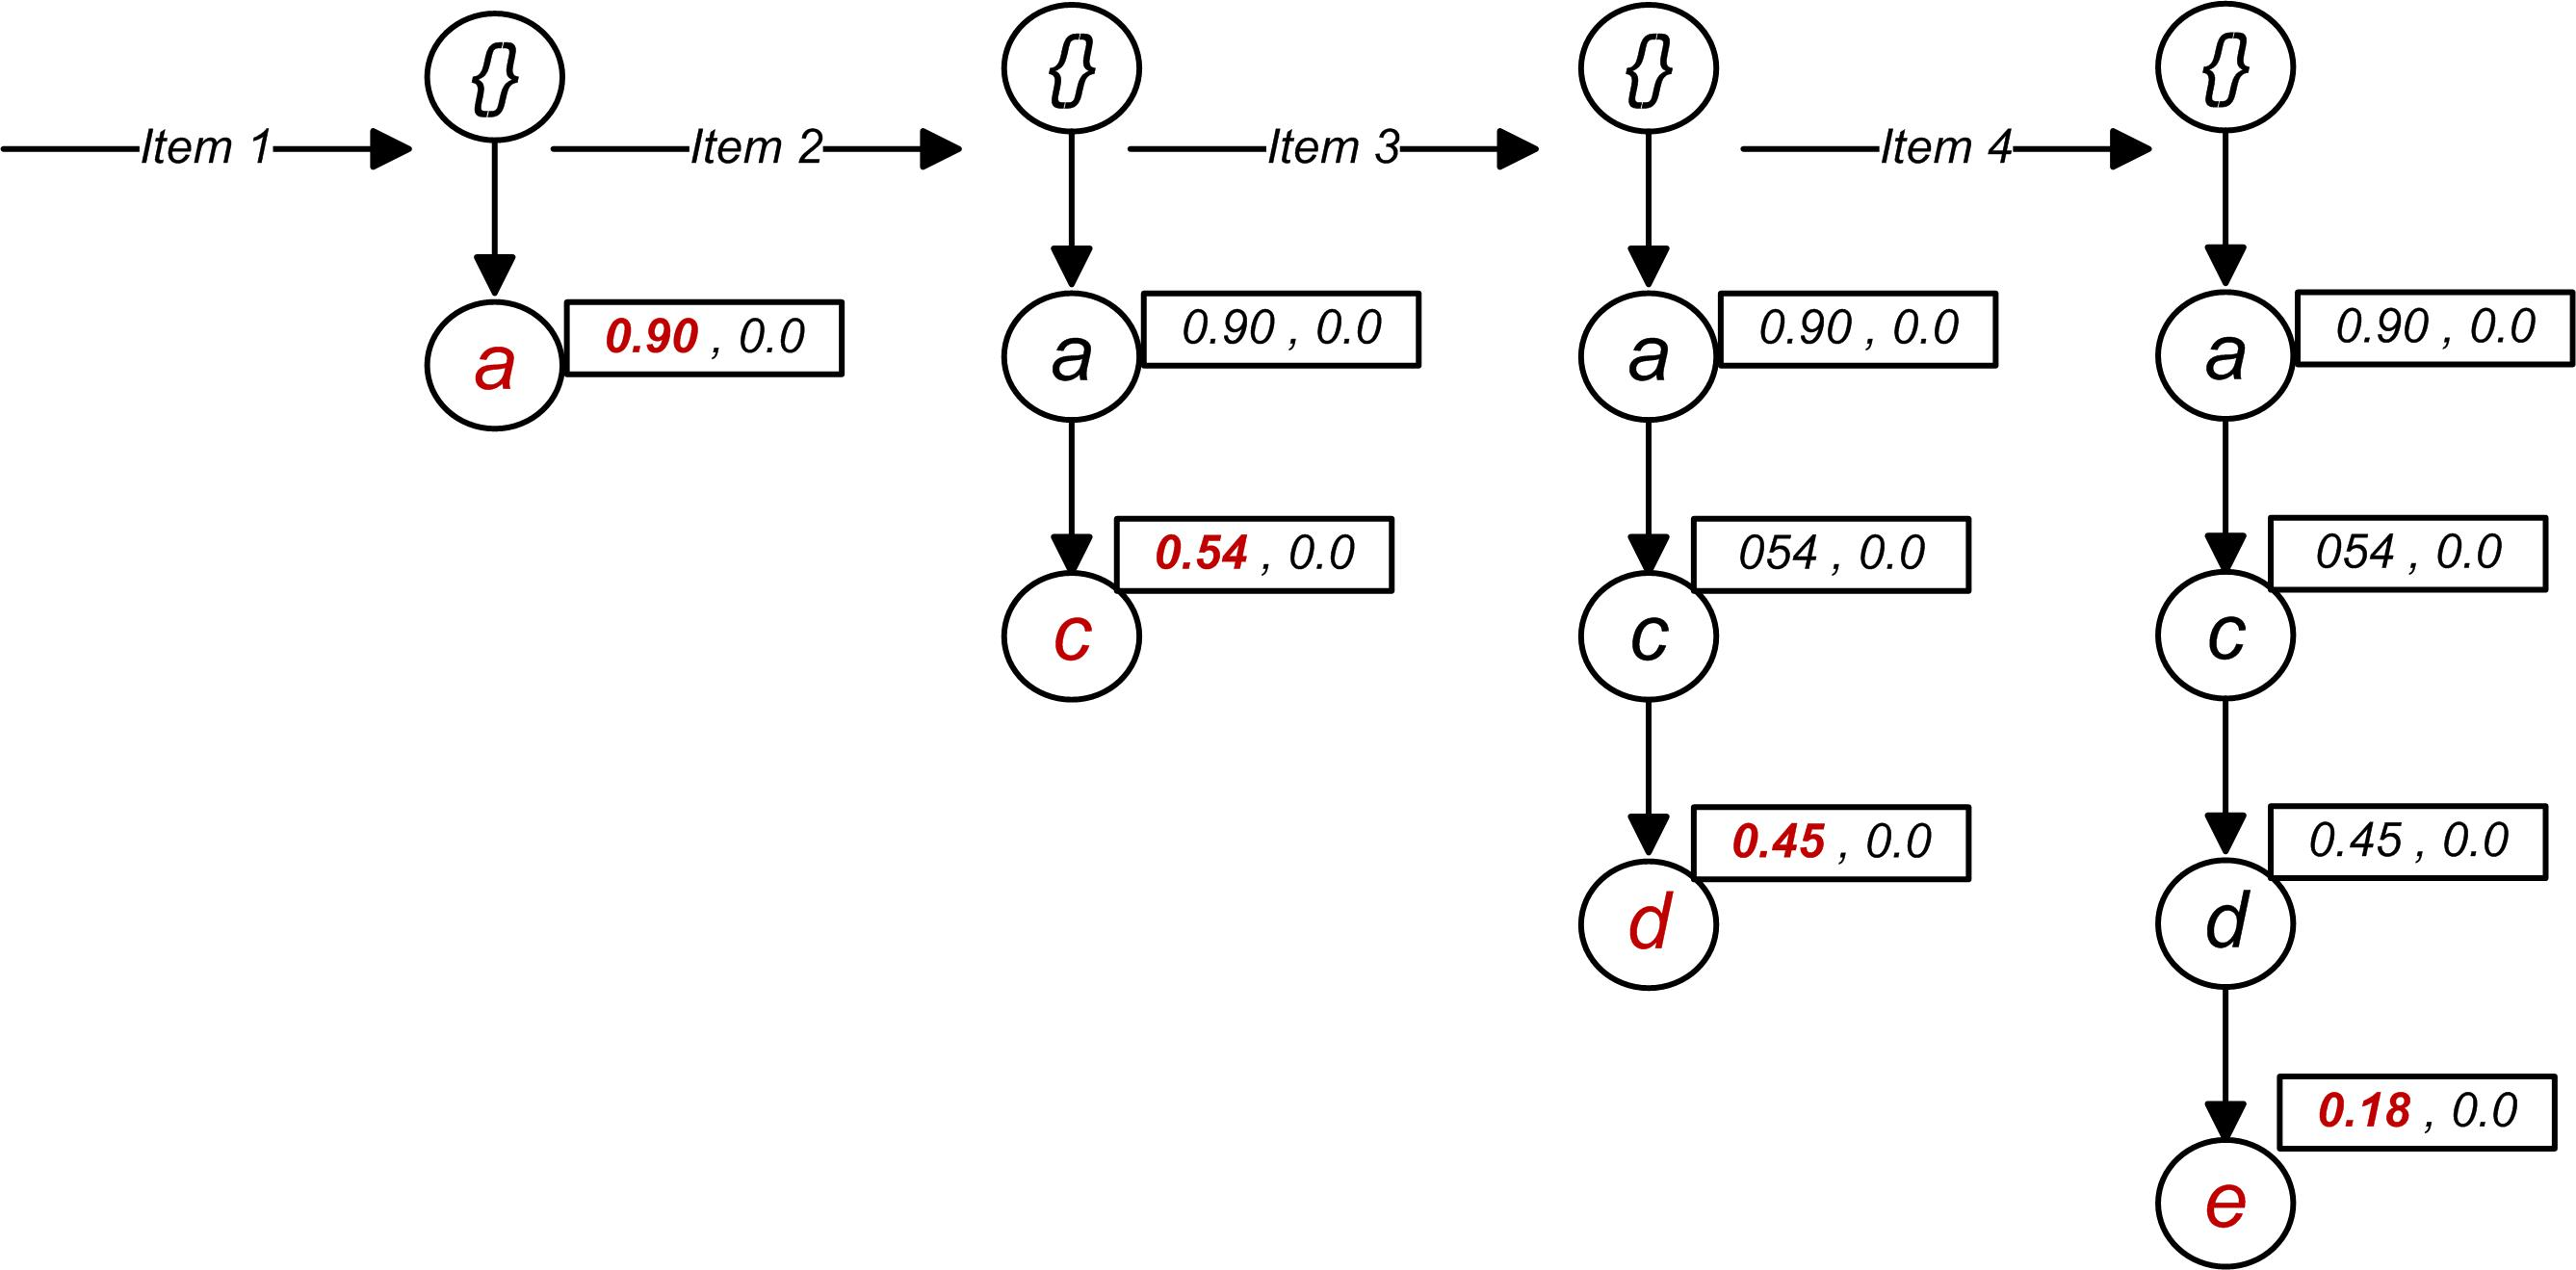
\includegraphics[width=\textwidth,height=3cm]{../images/sim_01.jpg}
	    \caption{T1}
		\end{subfigure}
	}
  \hfill
  	\fbox{  
	 	\begin{subfigure}[b]{0.27\textwidth}
	 	\centering
	    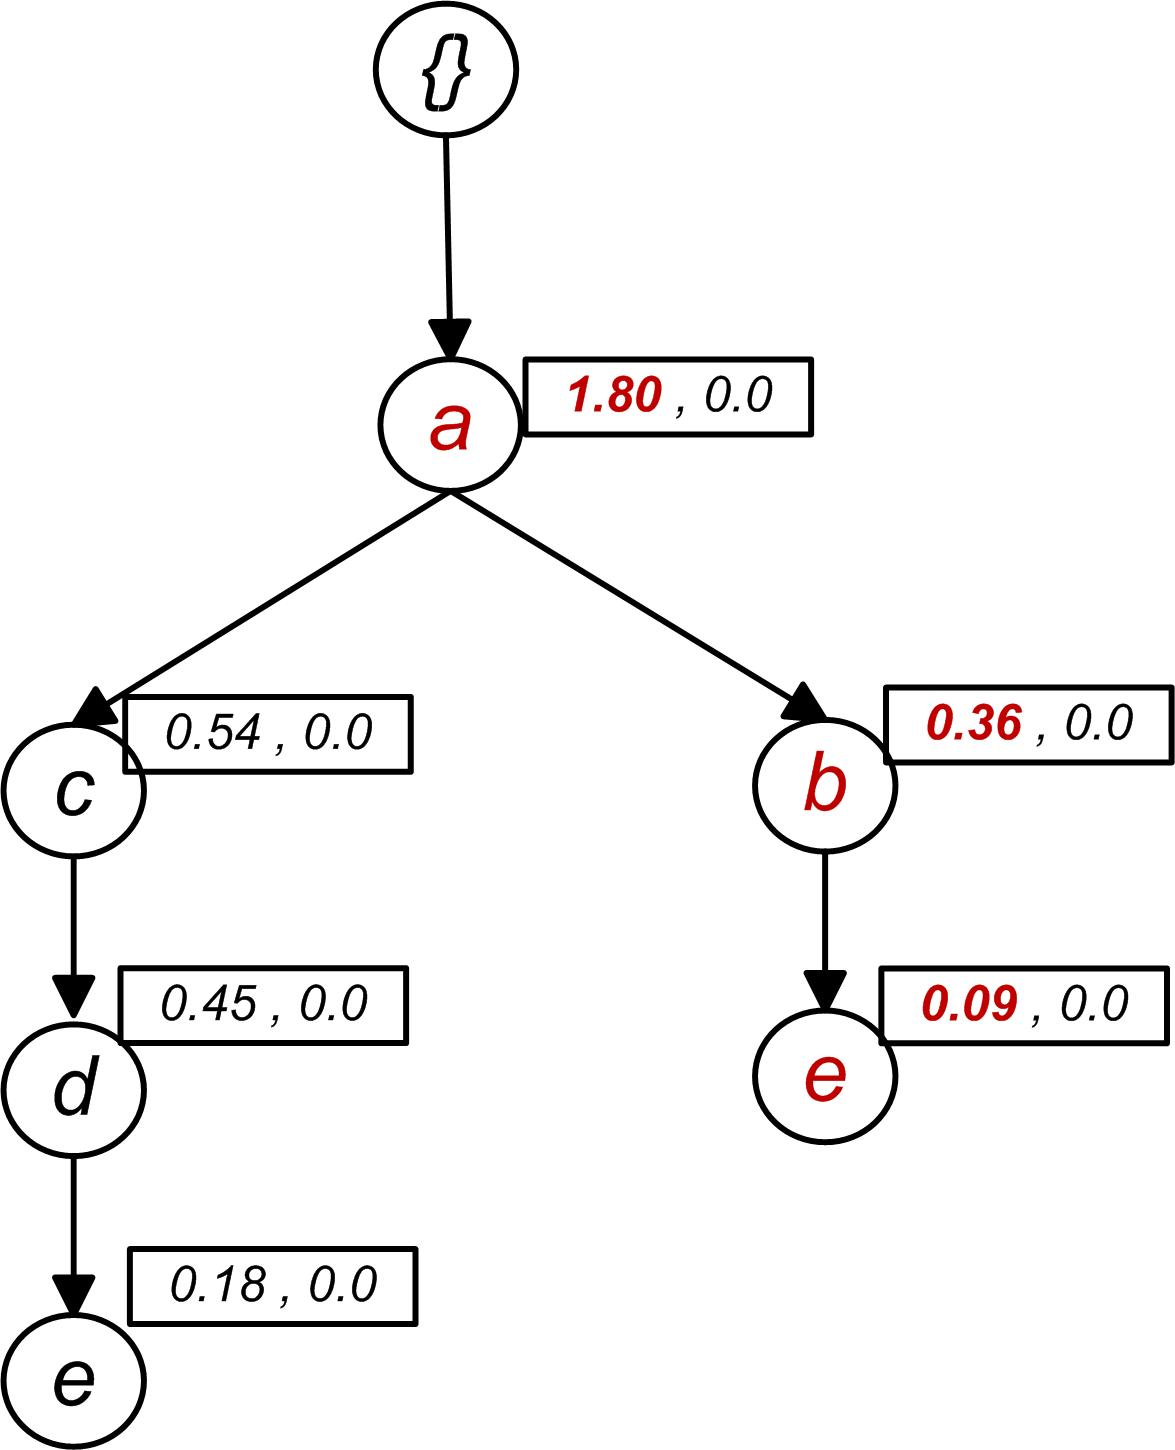
\includegraphics[width=\textwidth,height=3cm]{../images/sim_02.jpg}
	    \caption{T2}
		\end{subfigure}
	}
	\hfill
  \fbox{  
	 	\begin{subfigure}[b]{0.27\textwidth}
	 	\centering
	    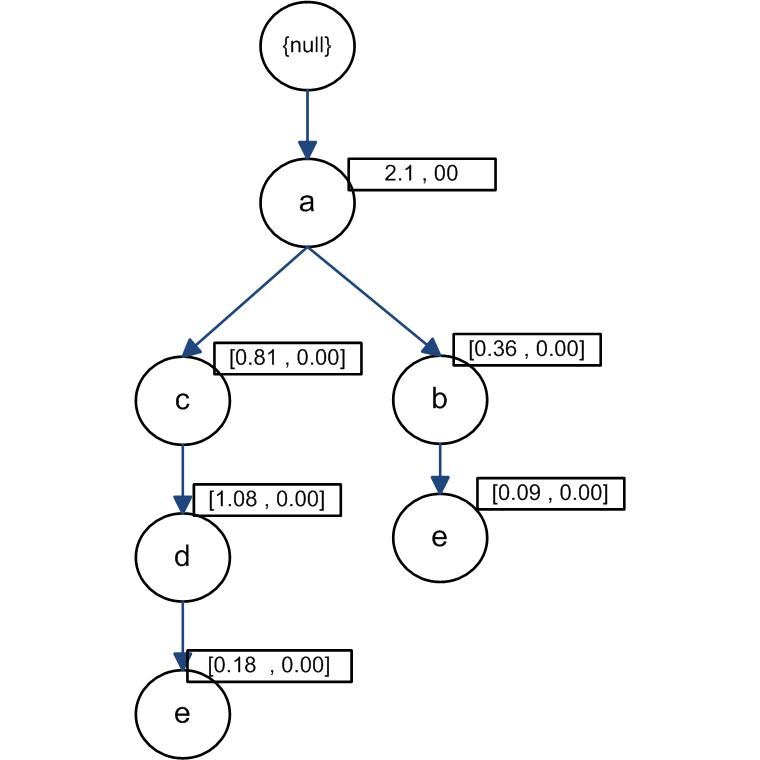
\includegraphics[width=\textwidth,height=3cm]{../images/sim_03.jpg}
	    \caption{T3}
		\end{subfigure}
	}
 \caption{Window 1}
\end{figure}
\end{frame}

\begin{frame}

\begin{figure}[!tbp]
  \centering
	\fbox{  
	 	\begin{subfigure}[b]{0.27\textwidth}
	 	\centering
	    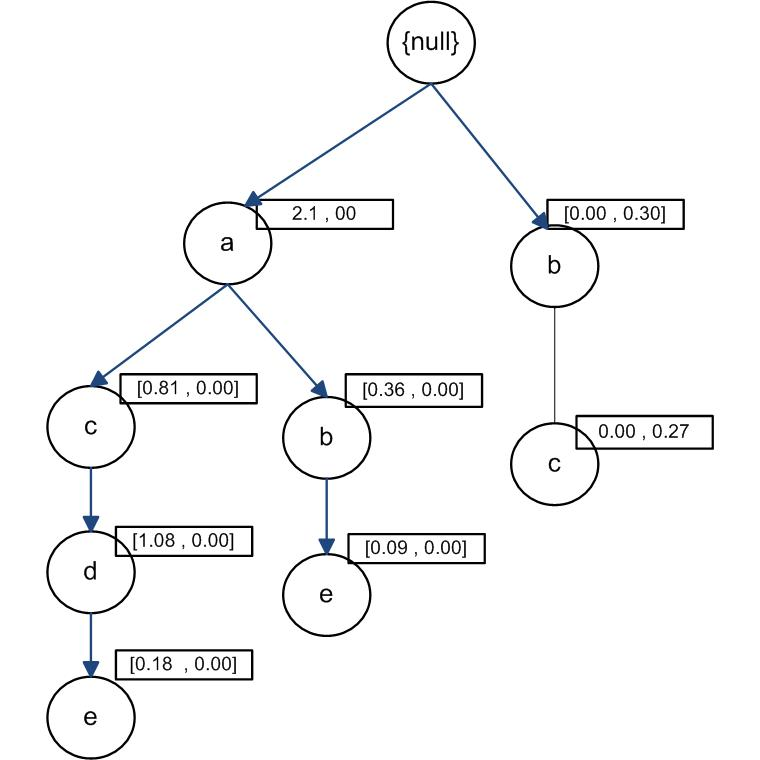
\includegraphics[width=\textwidth,height=3cm]{../images/sim_04.jpg}
	    \caption{T4}
		\end{subfigure}
	}
  \hfill
  	\fbox{  
	 	\begin{subfigure}[b]{0.27\textwidth}
	 	\centering
	    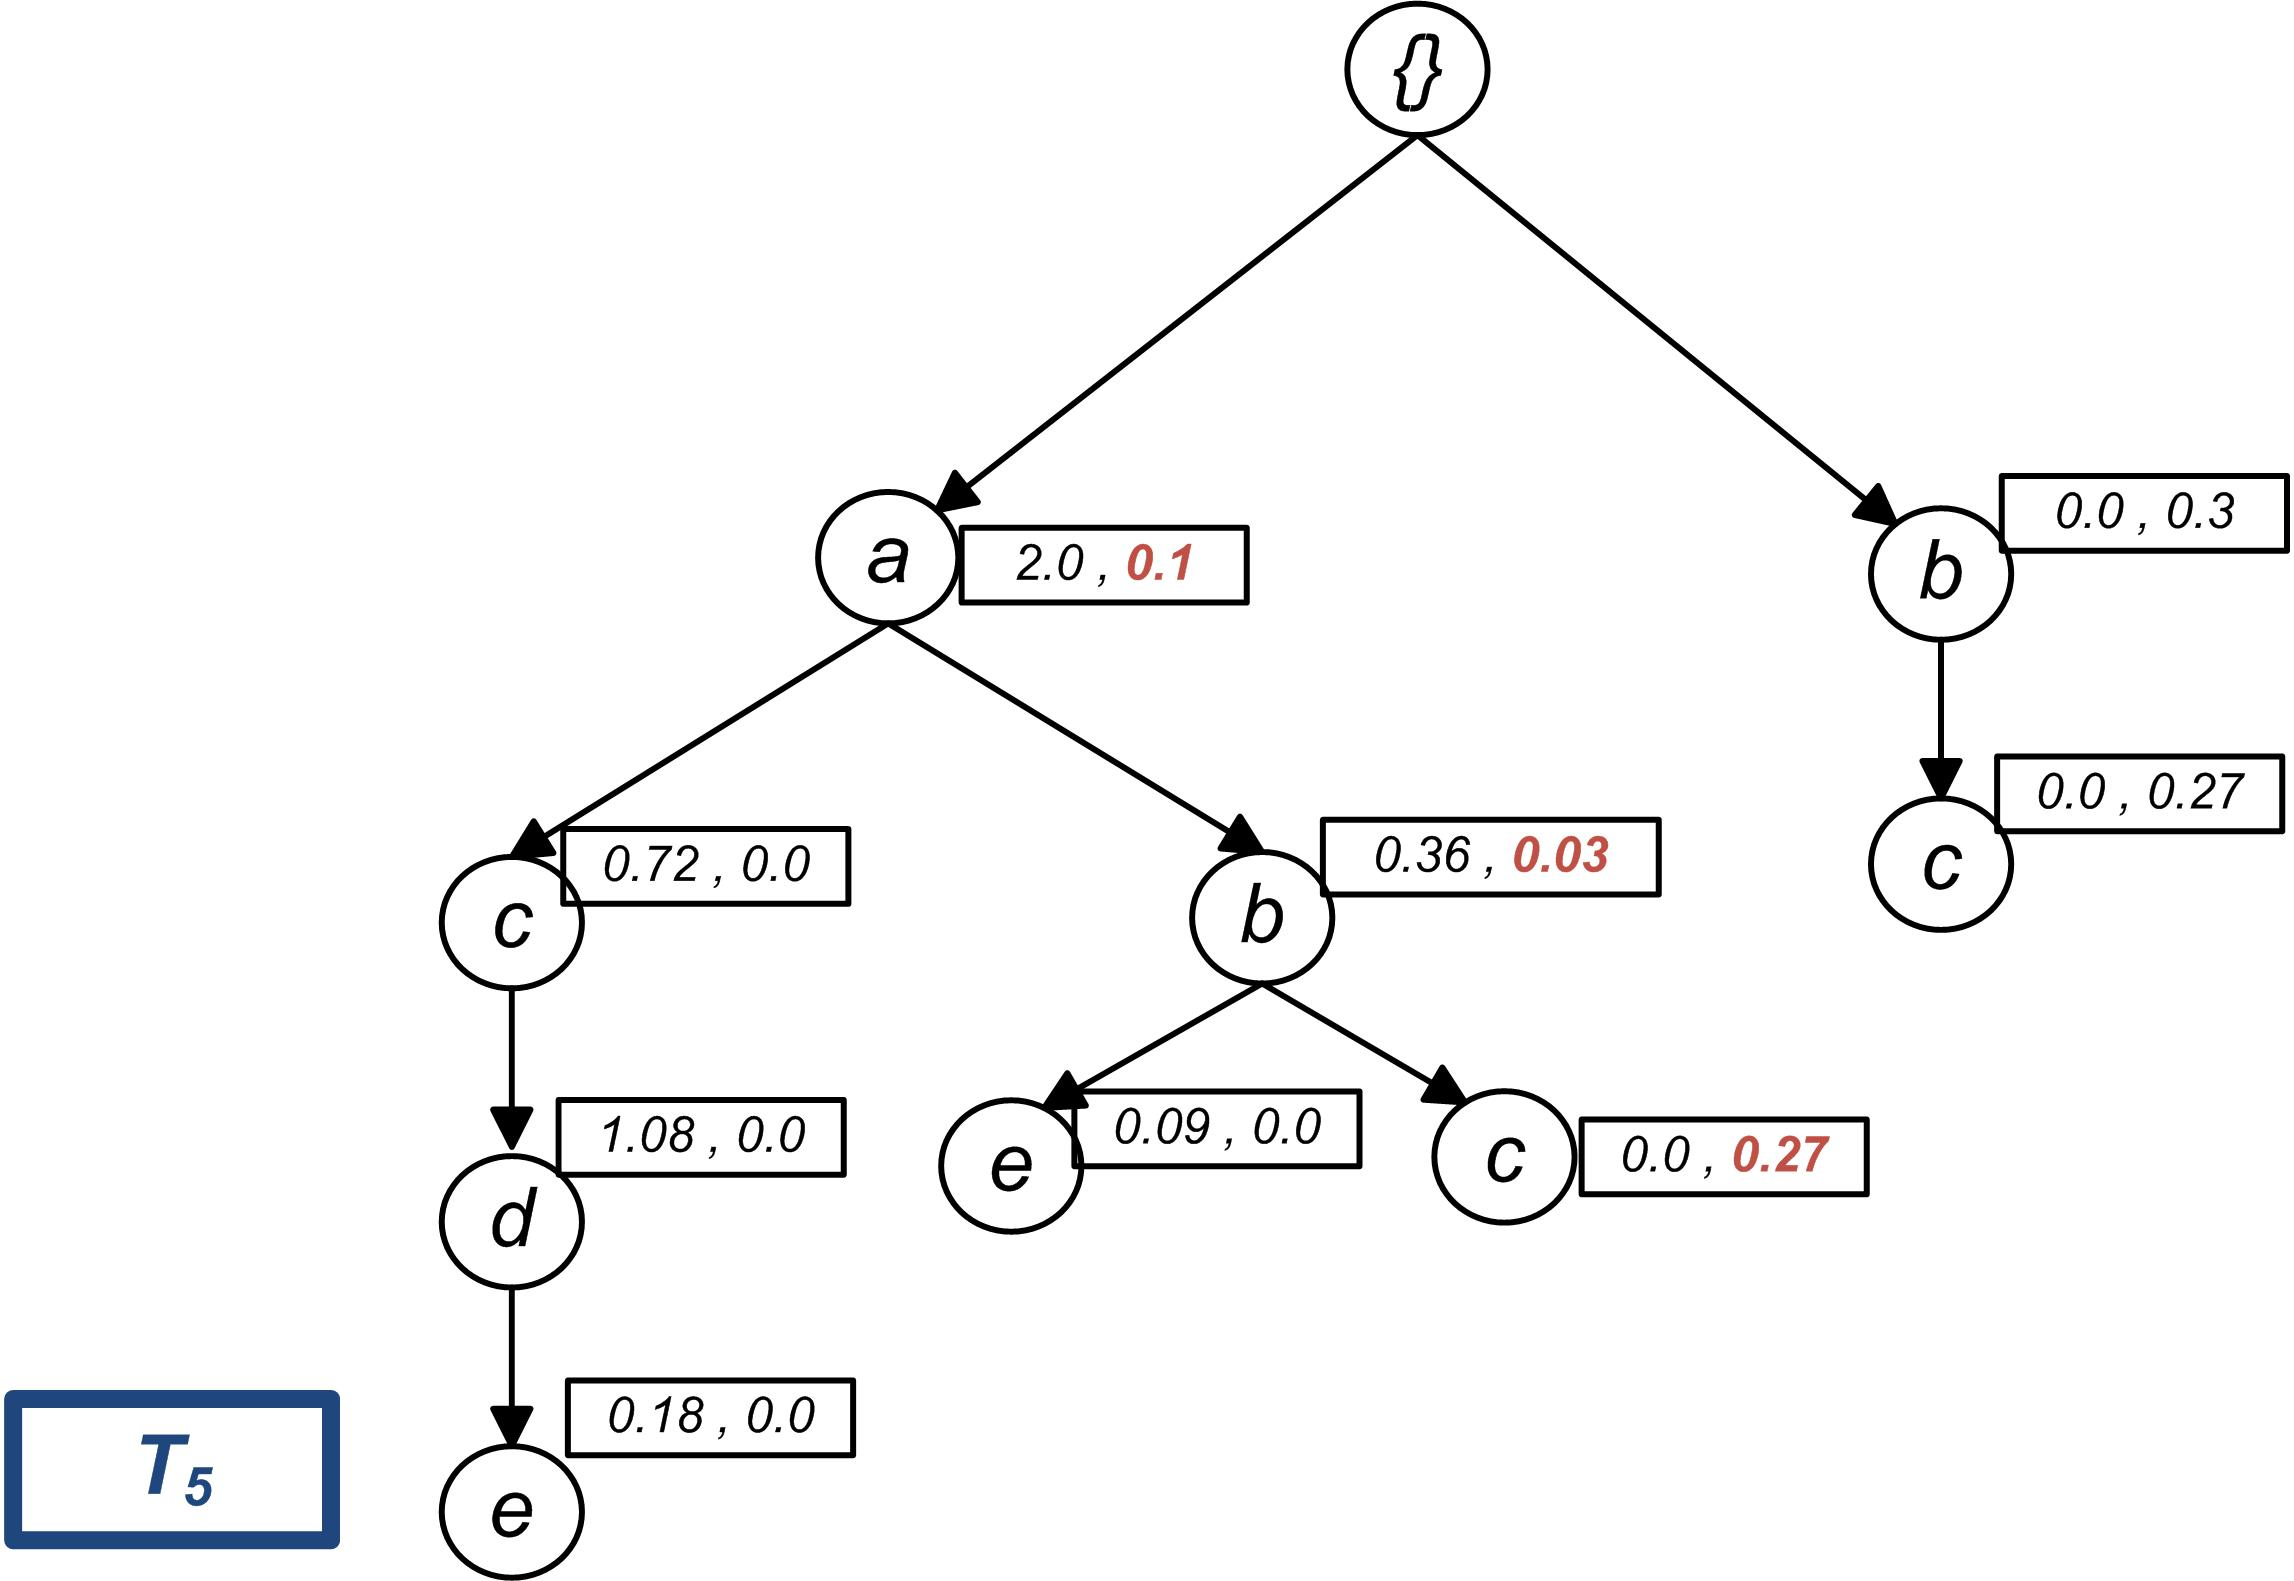
\includegraphics[width=\textwidth,height=3cm]{../images/sim_05.jpg}
	    \caption{T5}
		\end{subfigure}
	}
	\hfill
  \fbox{  
	 	\begin{subfigure}[b]{0.27\textwidth}
	 	\centering
	    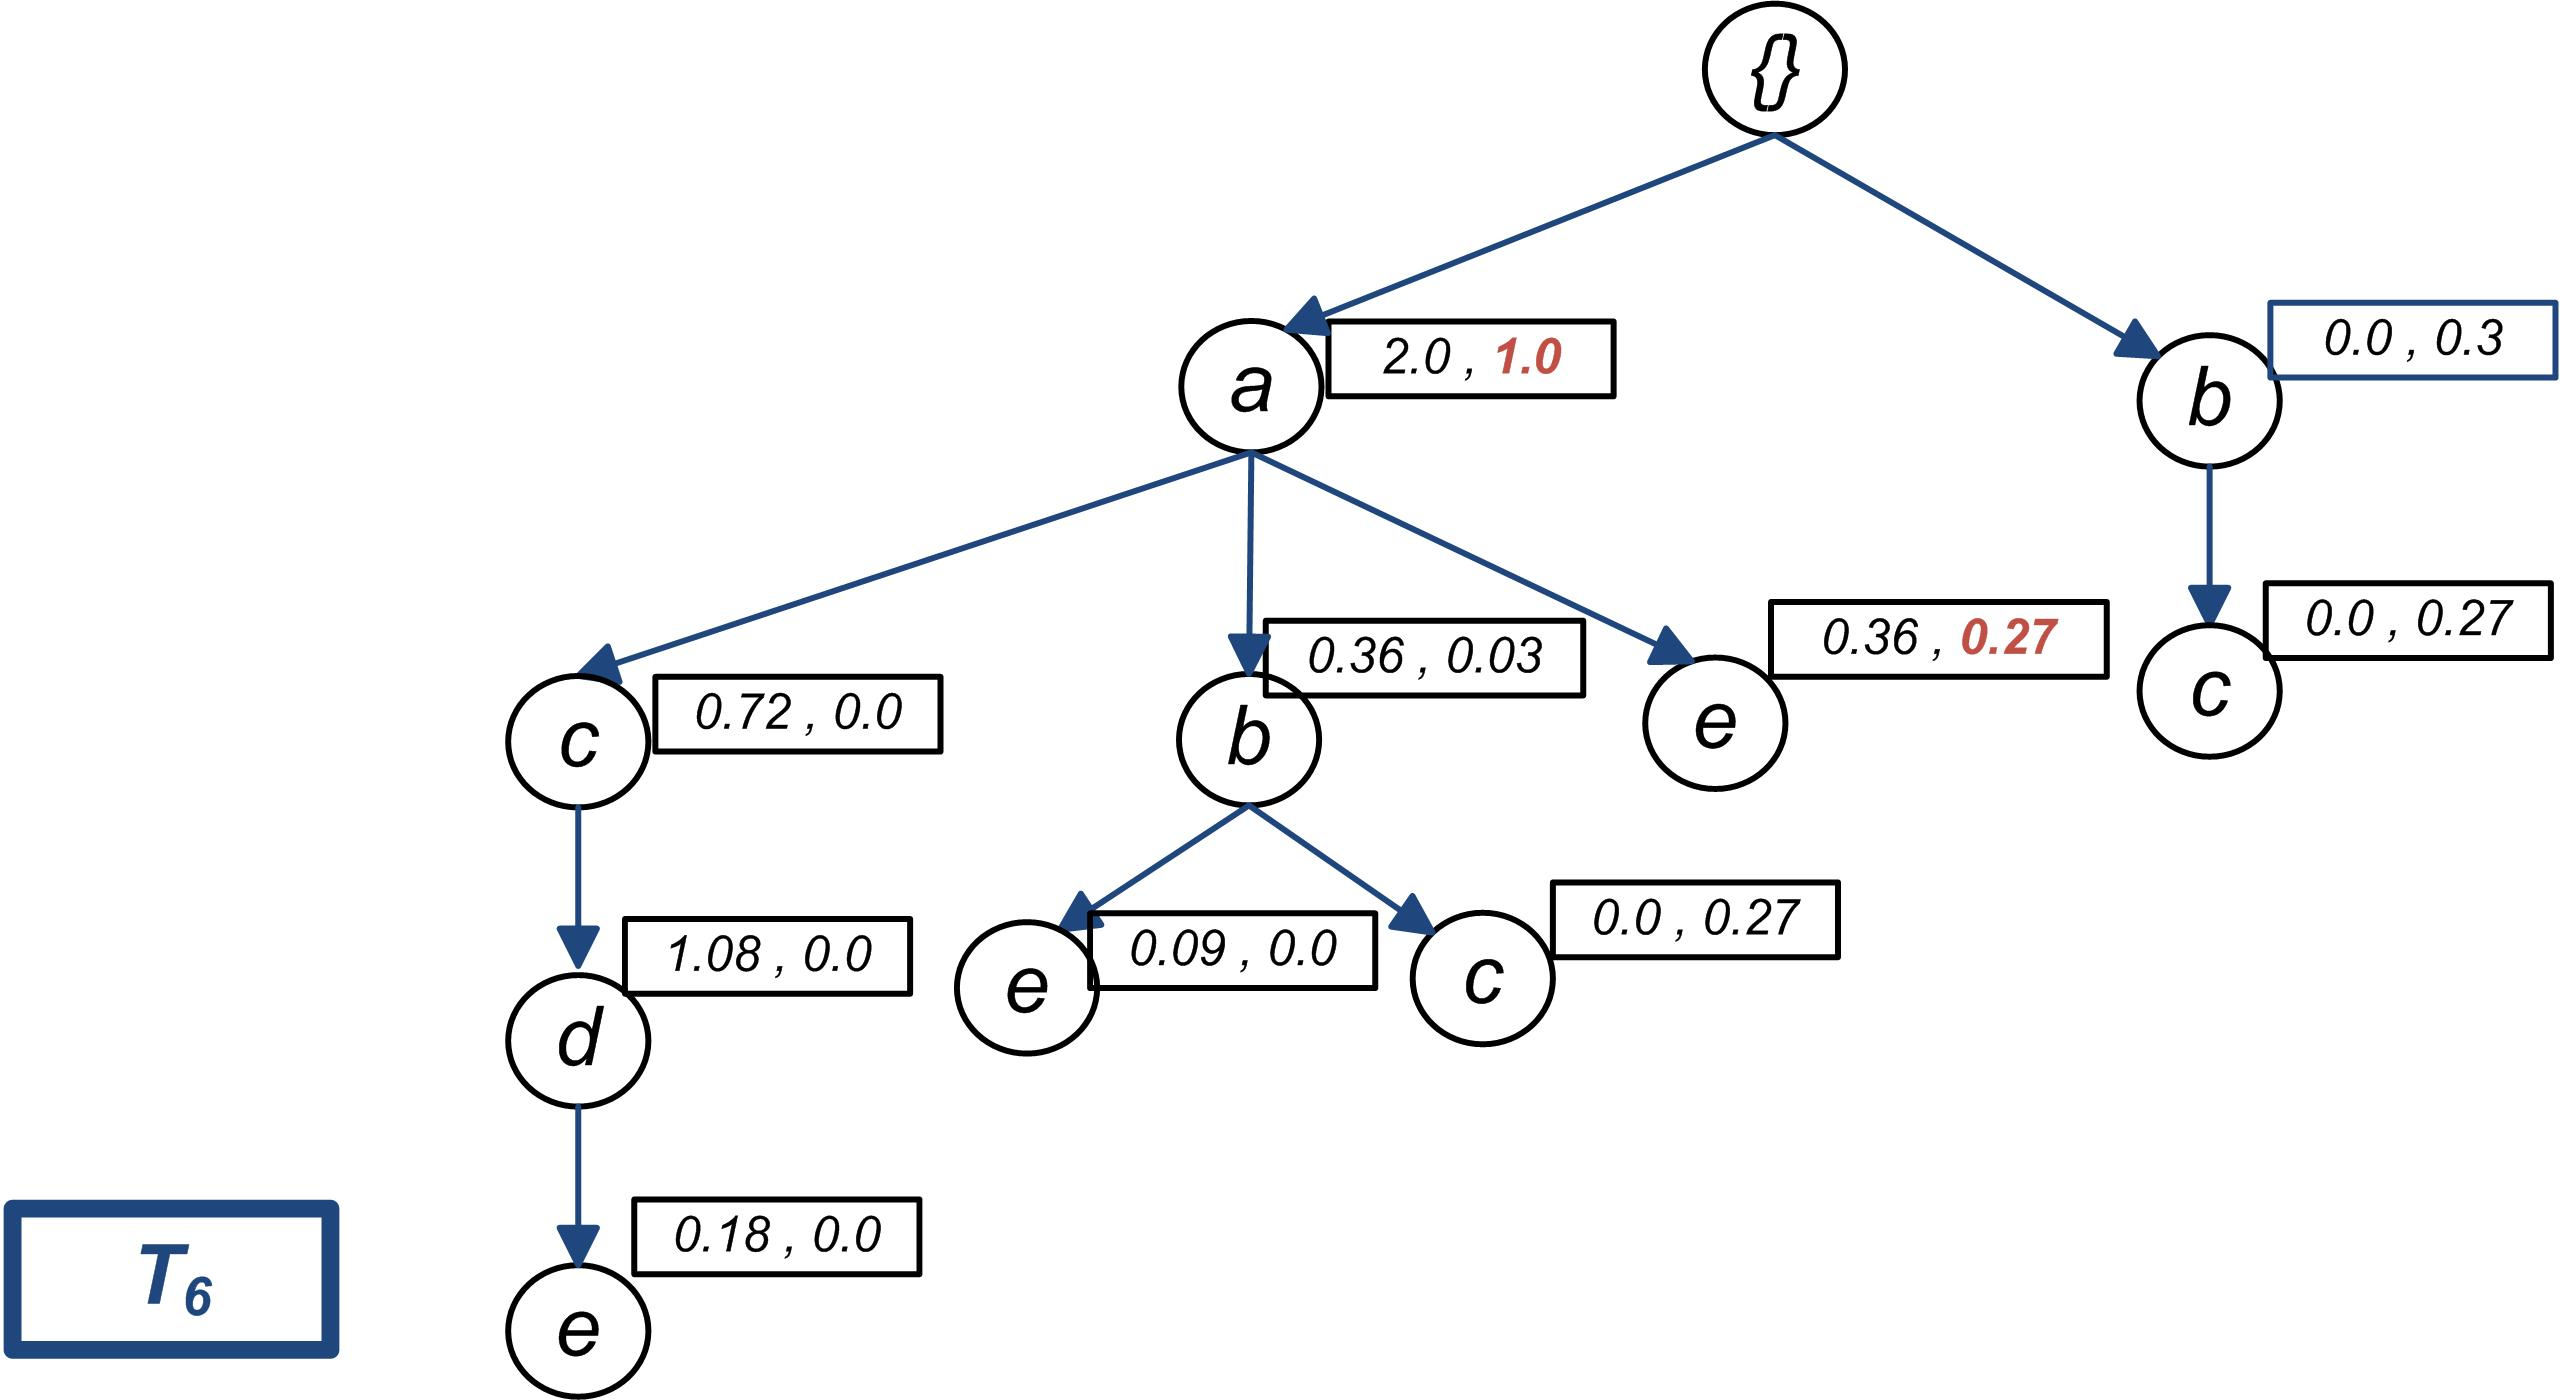
\includegraphics[width=\textwidth,height=3cm]{../images/sim_06.jpg}
	    \caption{T6}
		\end{subfigure}
	}
 \caption{Window 2}
\end{figure}
\end{frame}

\begin{frame}

\begin{figure}[!tbp]
  \centering
	\fbox{  
	 	\begin{subfigure}[b]{0.45\textwidth}
	 	\centering
	    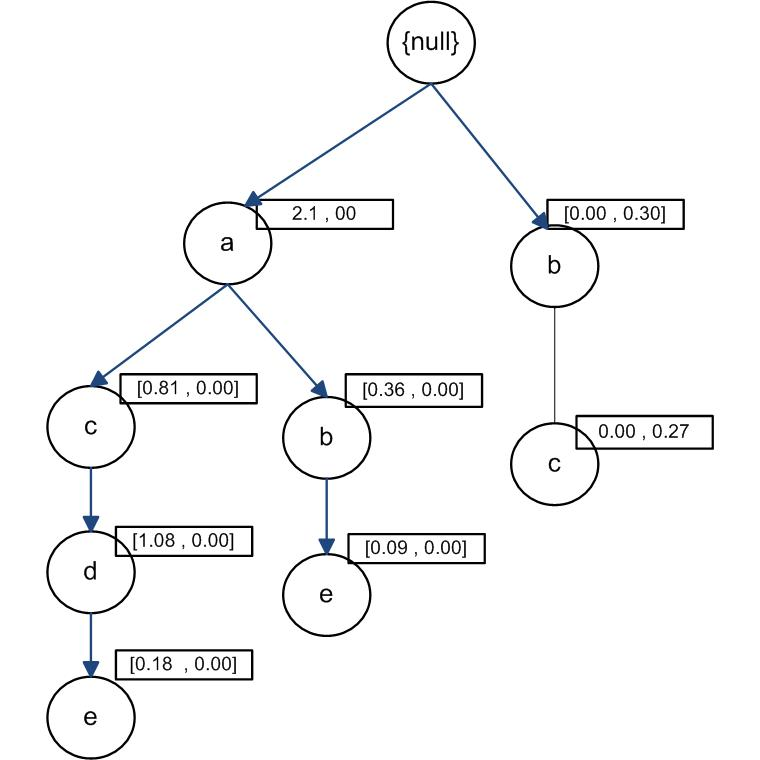
\includegraphics[width=\textwidth,height=5.5cm]{../images/sim_04.jpg}
	    \caption{Completed Window}
		\end{subfigure}
	}
  \hfill
  	\fbox{  
	 	\begin{subfigure}[b]{0.45\textwidth}
	 	\centering
	    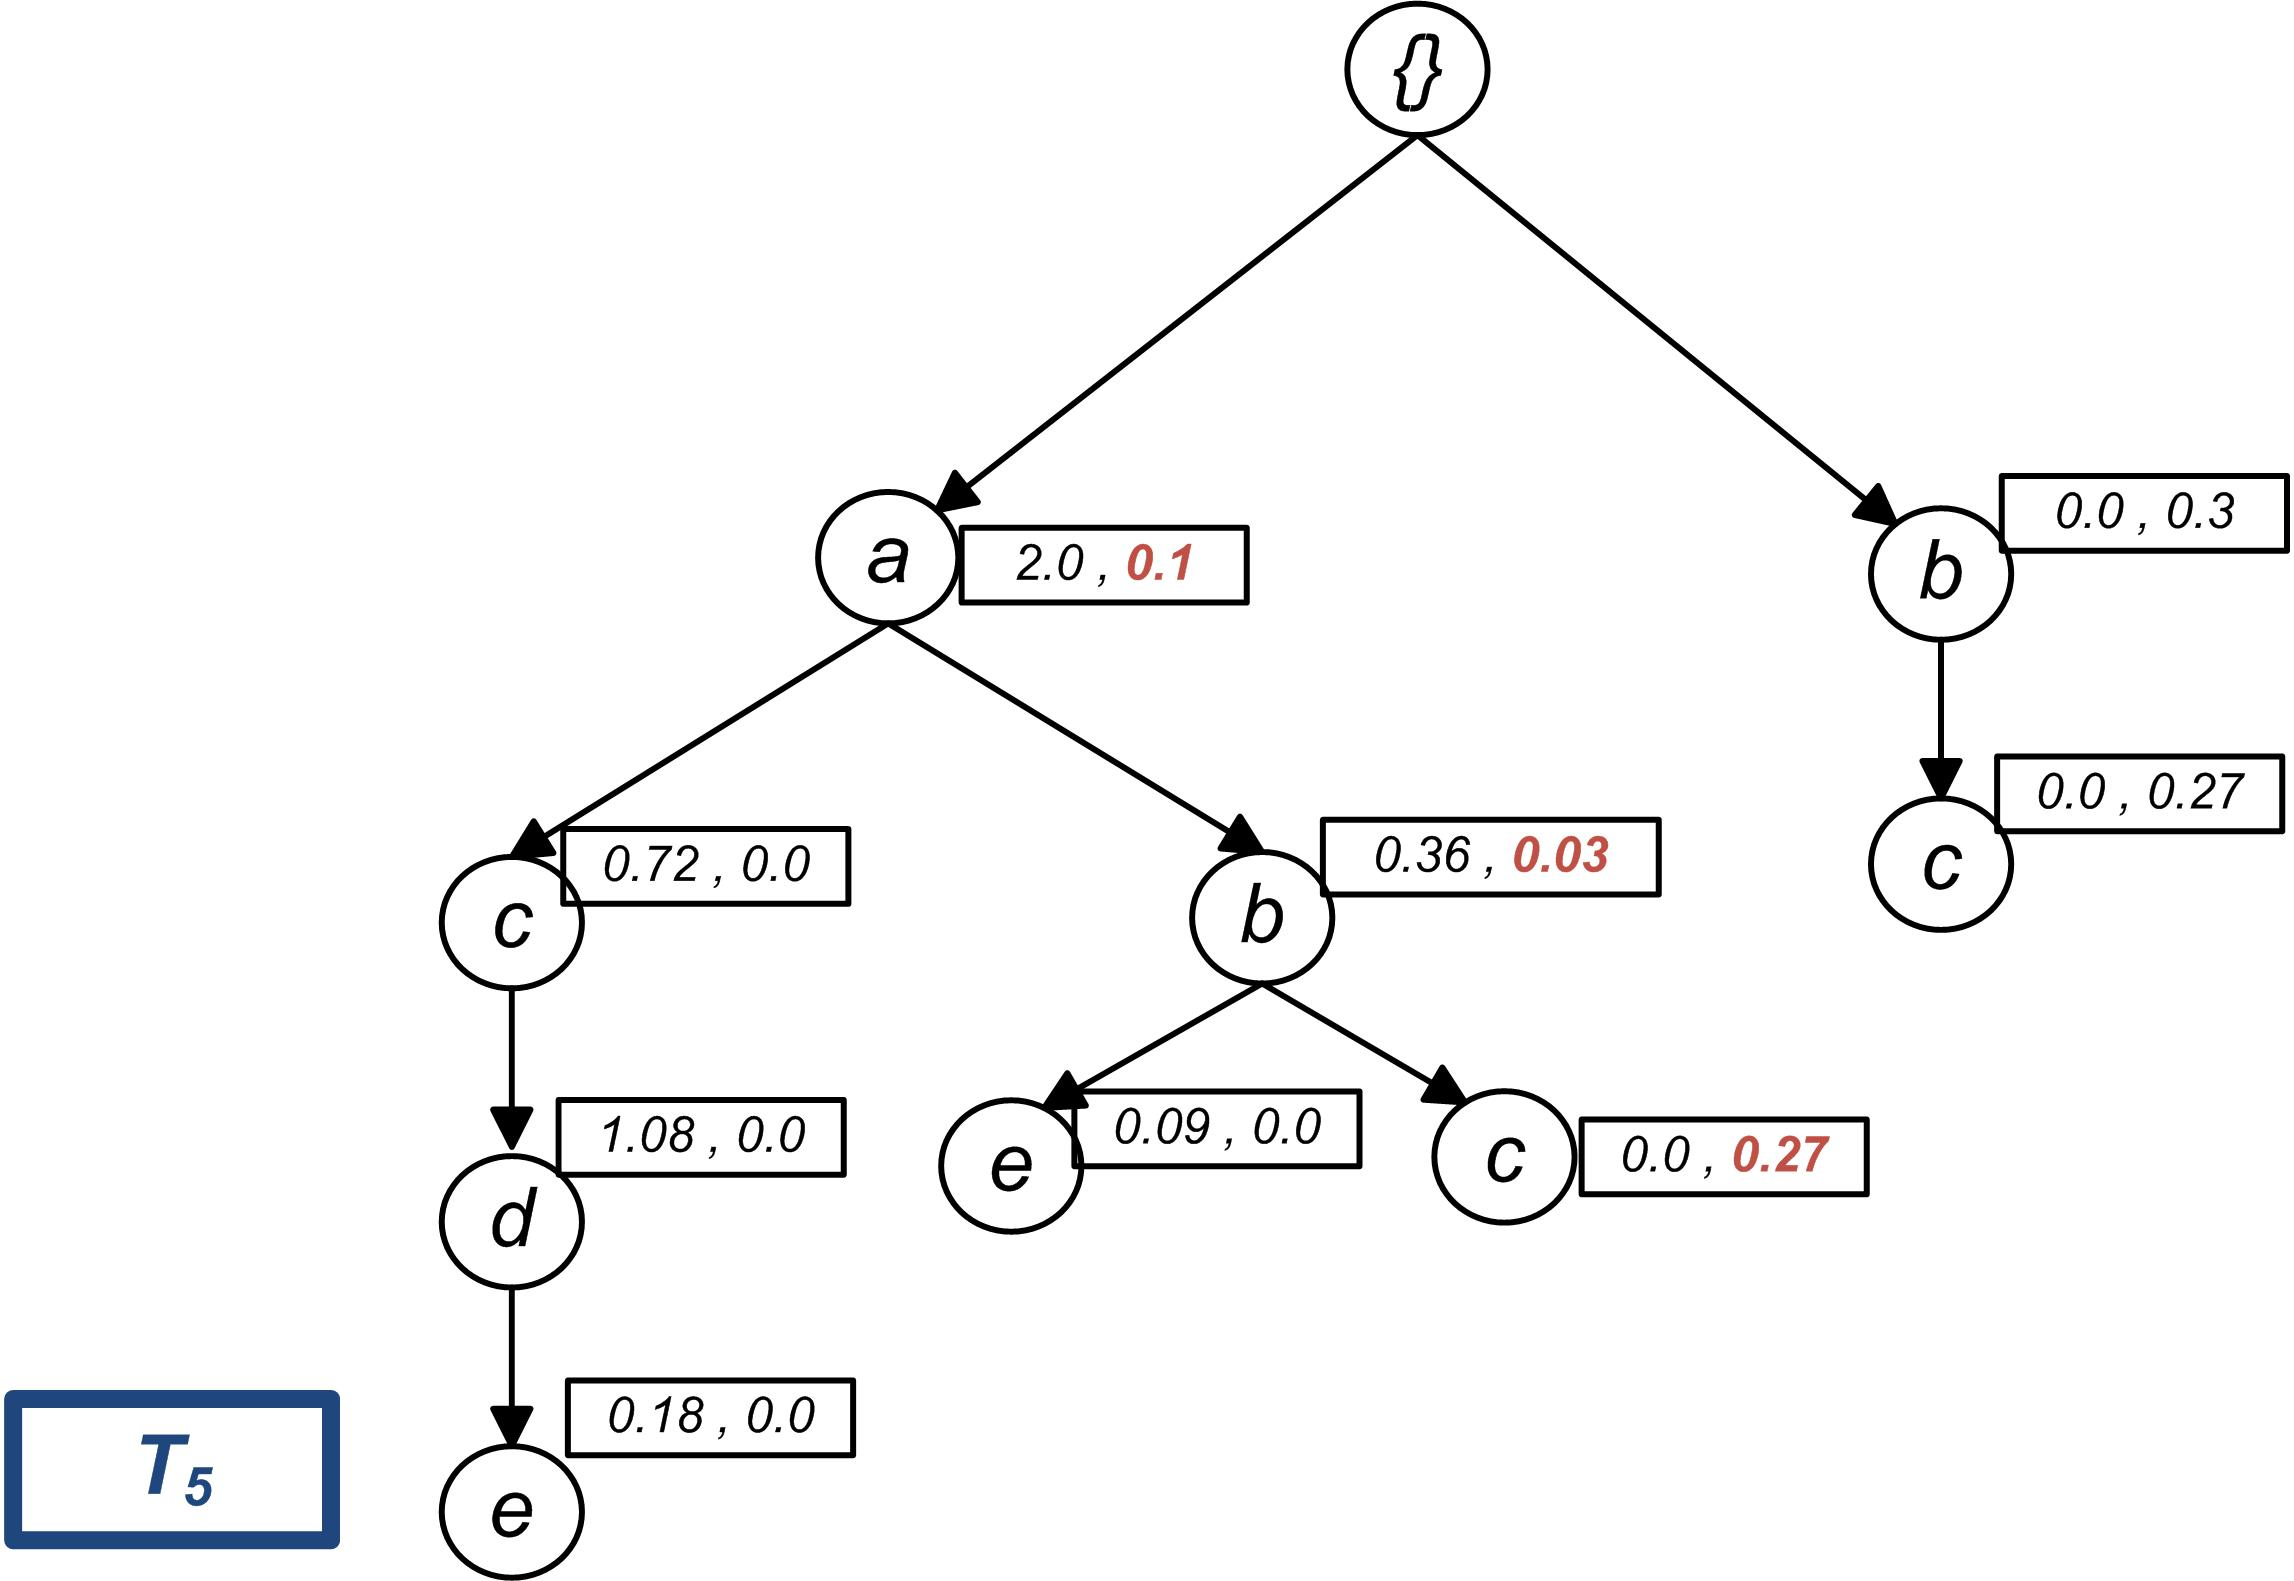
\includegraphics[width=\textwidth,height=5.5cm]{../images/sim_05.jpg}
	    \caption{Window after Slide}
		\end{subfigure}
	}
	\hfill
  
 \caption{After Sliding Window 2}
\end{figure}
\end{frame}

\end{document}
\paragraph*{}
In this section we will describe about our tree construction \emph{US-tree}. We have describe earlier about our batch and window. A batch should be inserted into the tree in it's own window slot. After inserting all batches of to full the window, the window shall be complete and be ready to mine. We said earlier section that our tree will be very compact. For this we have proposed an approach for sharing nodes. For sharing same tree nodes two items with same id and order should not care about own existential probability. If item is already in the tree with same id then two items should share the node. Thus the tree will be very compact.When inserting an item in the tree the \emph{U\textsuperscript{cap}}  of the tree should be updated by adding the prefix value of the node. Thus each batch should be inserted into the tree. 
\paragraph*{}
FOR EXAMPLE TABLE REF. First we insert \emph{Batch-1 (T\textsubscript{1}, T\textsubscript{2}, T\textsubscript{3})} in the window 1. As FIG WIN BATCH PLACEMENT 4 As the prefix has been calculated in TABLE REF for easy understanding the simulation we shall use this table to simulate. First when inserting the \emph{T\textsubscript{1} - a(0.9), c(0.54), d(0.45), e(0.18)} we insert item \emph{a(0.9)} as a child of root \emph{\{\}}. Update a's prefix value as $0.9$. Then we add \emph{c(0.54)} as a's child update c's prefix value as $0.54$. Aad \emph{d(0.45)} as c's child update d's prefix value as $0.45$. Add \emph{e(0.18)} as d's child update e's prefix value as $0.18$. Thus \emph{T1} is inserted into the tree. For \emph{T\textsubscript{2} - a(0.9), b(0.36), e(0.09)} first we insert \emph{a(0.9)}. Here we found \emph{a} is already inserted so we just update existing node a's prefix value $0.9 + 0.9 = 1.8$. Then we insert \emph{b(0.36)}. As \emph{a} has no child \emph{b} we insert a new child b and update it's prefix value $0.36$. Then insert new e(0.09) as the child of \emph{b}. For \emph{T\textsubscript{3} - a(0.2), c(0.18), d(0.63)} we follow the existing path \emph{a(1.8), c(0.54), d(0.45)} and update corresponding prefix value as $1.8 + 0.2 = 2.0$, $0.54 + 0.18 = 0.72$ and $0.45 + 0.63 = 1.08$. After inserting the This \emph{T\textsubscript{3}} window 1 is completed. Then we will go for inserting next batch \emph{Batch-2 (T\textsubscript{4}, T\textsubscript{5}, T\textsubscript{6})} in the tree. For \emph{Batch-2} we shall put prefix value in the window's newest place. And thus the latest batch becomes the most recent information. For inserting \emph{T\textsubscript{4} - b(0.3), c(0.27)} we insert new node \emph{b} as there is no child b of root node \emph{\{\}}. So we insert \emph{b} as a child of root \emph{\{\}}. update its prefix value as $0.3$. Then insert \emph{c(0.27)} as child of \emph{b} and update prefix value $0.27$. Here as this \emph{T\textsubscript{4}} is inserting in \emph{Batch-4} we update prefix value for recent batch's information. Next we insert \emph{T\textsubscript{5} - a(0.1), b(0.03), c(0.27)}. 
We merge \emph{a(0.1), b(0.03)} with previous \emph{a, b } nodes and update prefix value $0.1$ and $0.03$ in the second batch's portion and insert new node \emph{b} as a child of \emph{b} and update its prefix value as $0.27$.



%\end{document}
\subsection{Sliding Window}
%\documentclass{article}
%\begin{document}
\paragraph*{}
In this section we will describe elaborately about our mining procedure. An important fact in our data type is transaction comes in as a stream and that's why we have created a window based 
%\end{document}


\subsection{Mining US-tree : FPUS-growth}
%\documentclass{article}
%\usepackage{caption}
%\usepackage{graphicx}
%\begin{document}


%
%%\documentclass{article}
%\usepackage{caption}
%\usepackage{graphicx}
%\begin{document}

\end{document}

%\documentclass{article}
%\usepackage{caption}
%\usepackage{graphicx}
%\begin{document}

\begin{figure}
\begin{minipage}{0.40\textwidth}
  \centering
  
	\begin{center}
	\begin{tabular}{ |c|c|c| } 
 	\hline
 		Item&\emph{U\textsuperscript{cap}}&Support\\ \hline\hline
 		a &  3.00  & 3.00	\\ \hline
 		c &  1.26  & 3.30	\\ \hline
 		d &  1.08  & 1.20	\\ \hline
 		e &  0.54  & 0.60	\\ \hline
 		b &  0.69  & 1.00	\\ \hline
\end{tabular}
\end{center}   
  \captionof{table}{Header Table of US-tree}
\end{minipage}
\hfill
\begin{minipage}{0.40\textwidth}
  \centering
  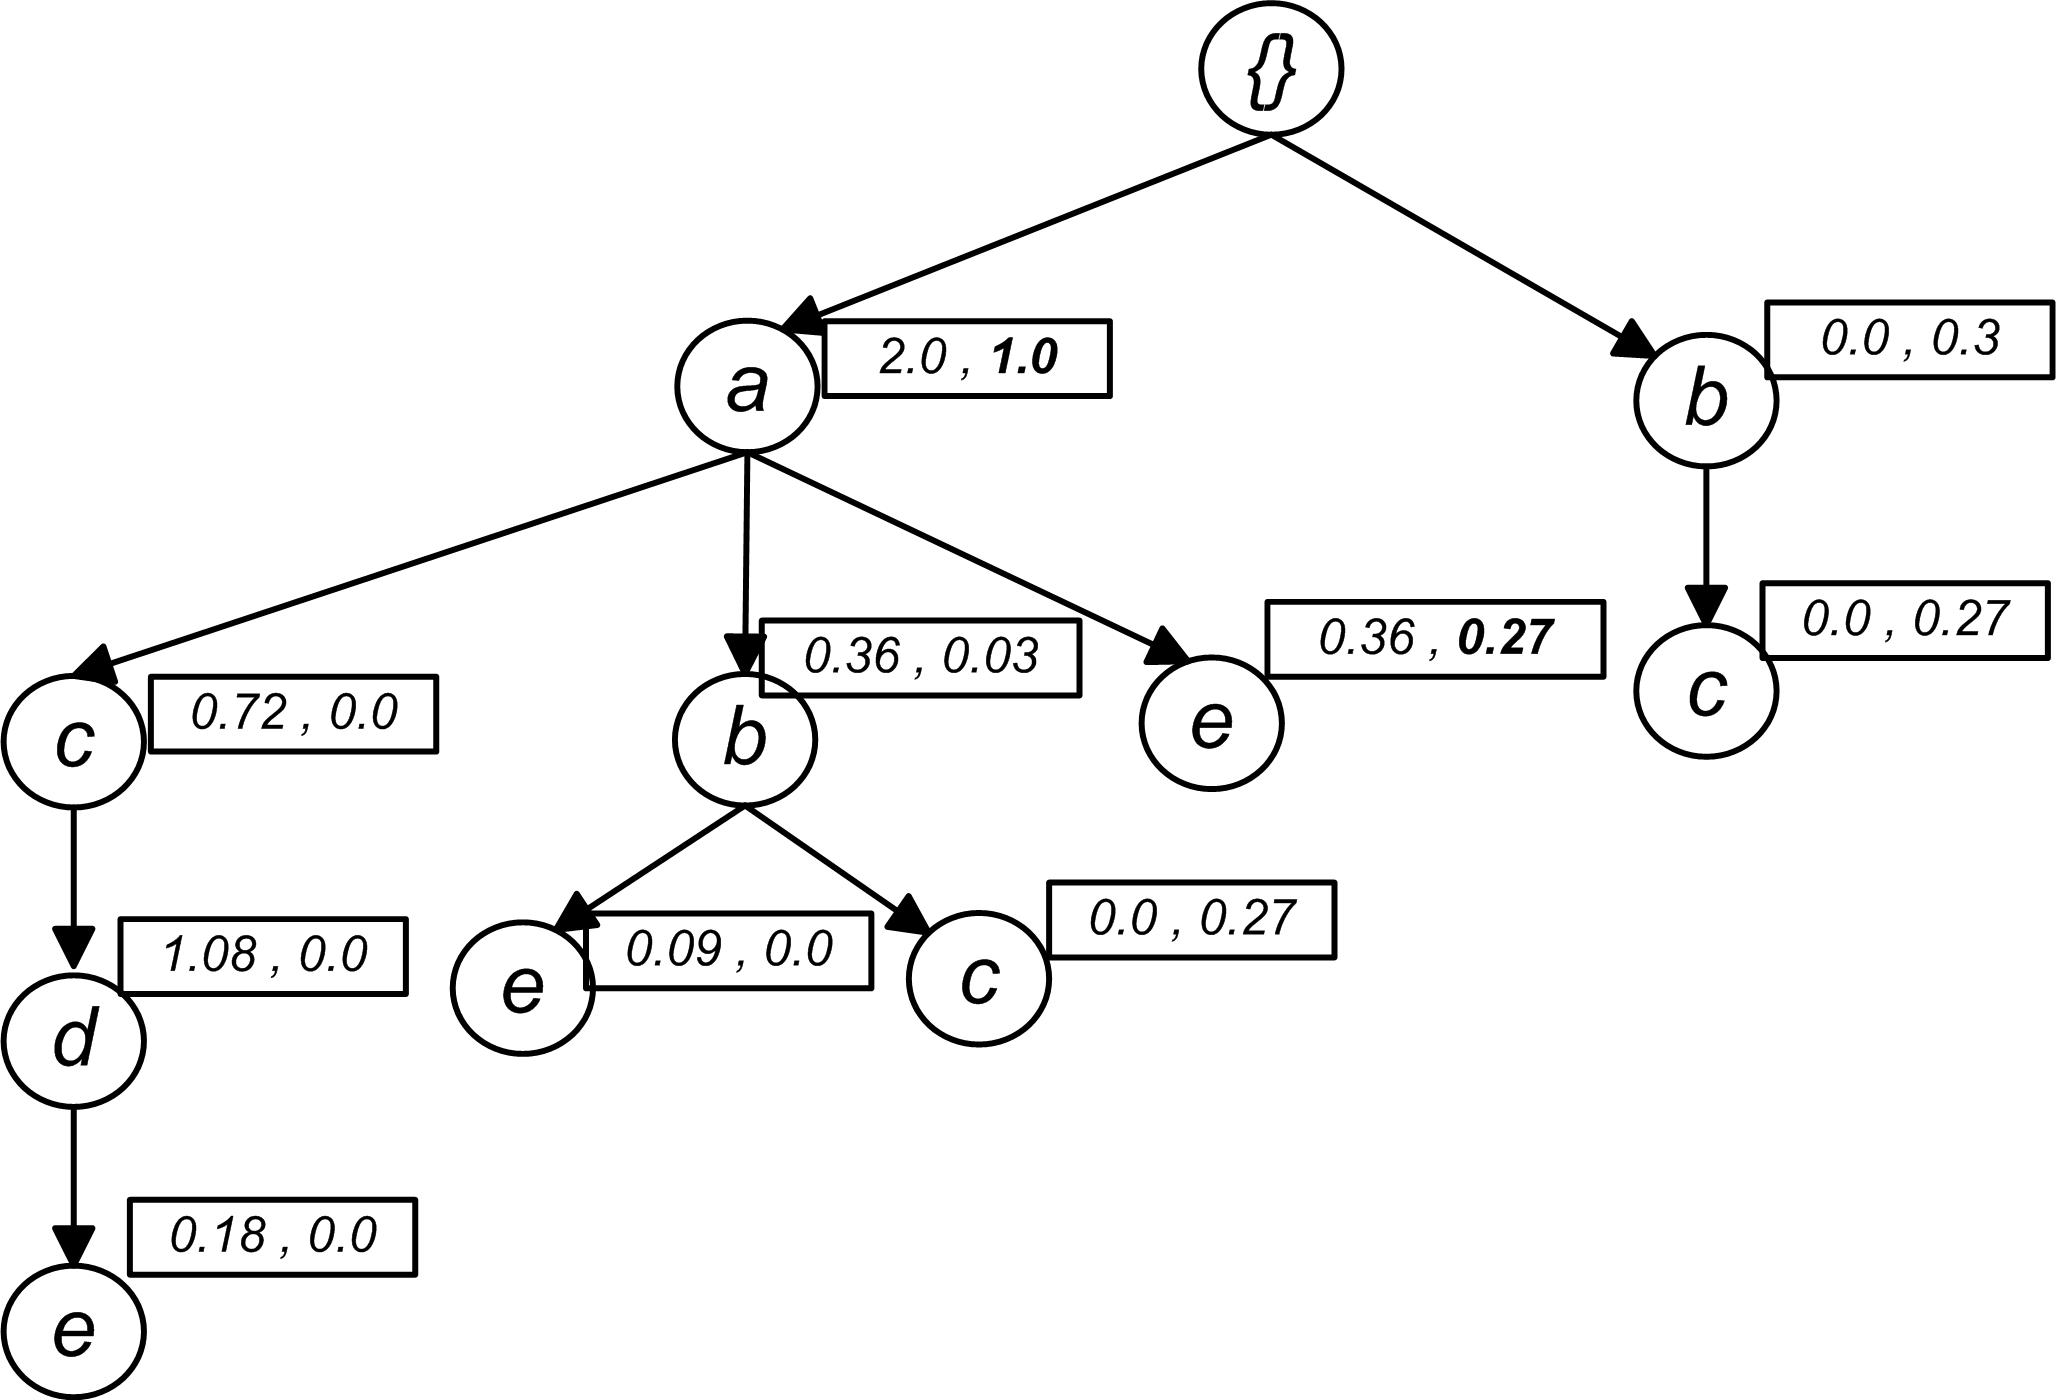
\includegraphics[width=\textwidth]{images/us_tree.jpg}
  \captionof{figure}{US-tree}
\end{minipage}
\caption{US-tree and Header Table}
\label{figure:min_before}
\end{figure}


\begin{figure}
\begin{minipage}{0.40\textwidth}
  \centering
  
	\begin{center}
	\begin{tabular}{ |c|c|c| } 
 	\hline
 		Item&\emph{U\textsuperscript{cap}}&Support\\ \hline\hline
 		a &  3.00  & 3.00\\ \hline
 		c &  1.26  & 3.30\\ \hline
 		d &  1.08  & 1.20\\ \hline
 		b &  0.69  & 1.00\\ \hline
\end{tabular}
\end{center}  
  
  
  \captionof{table}{Header Table for Mining}
\end{minipage}
\hfill
\begin{minipage}{0.40\textwidth}
  \centering
  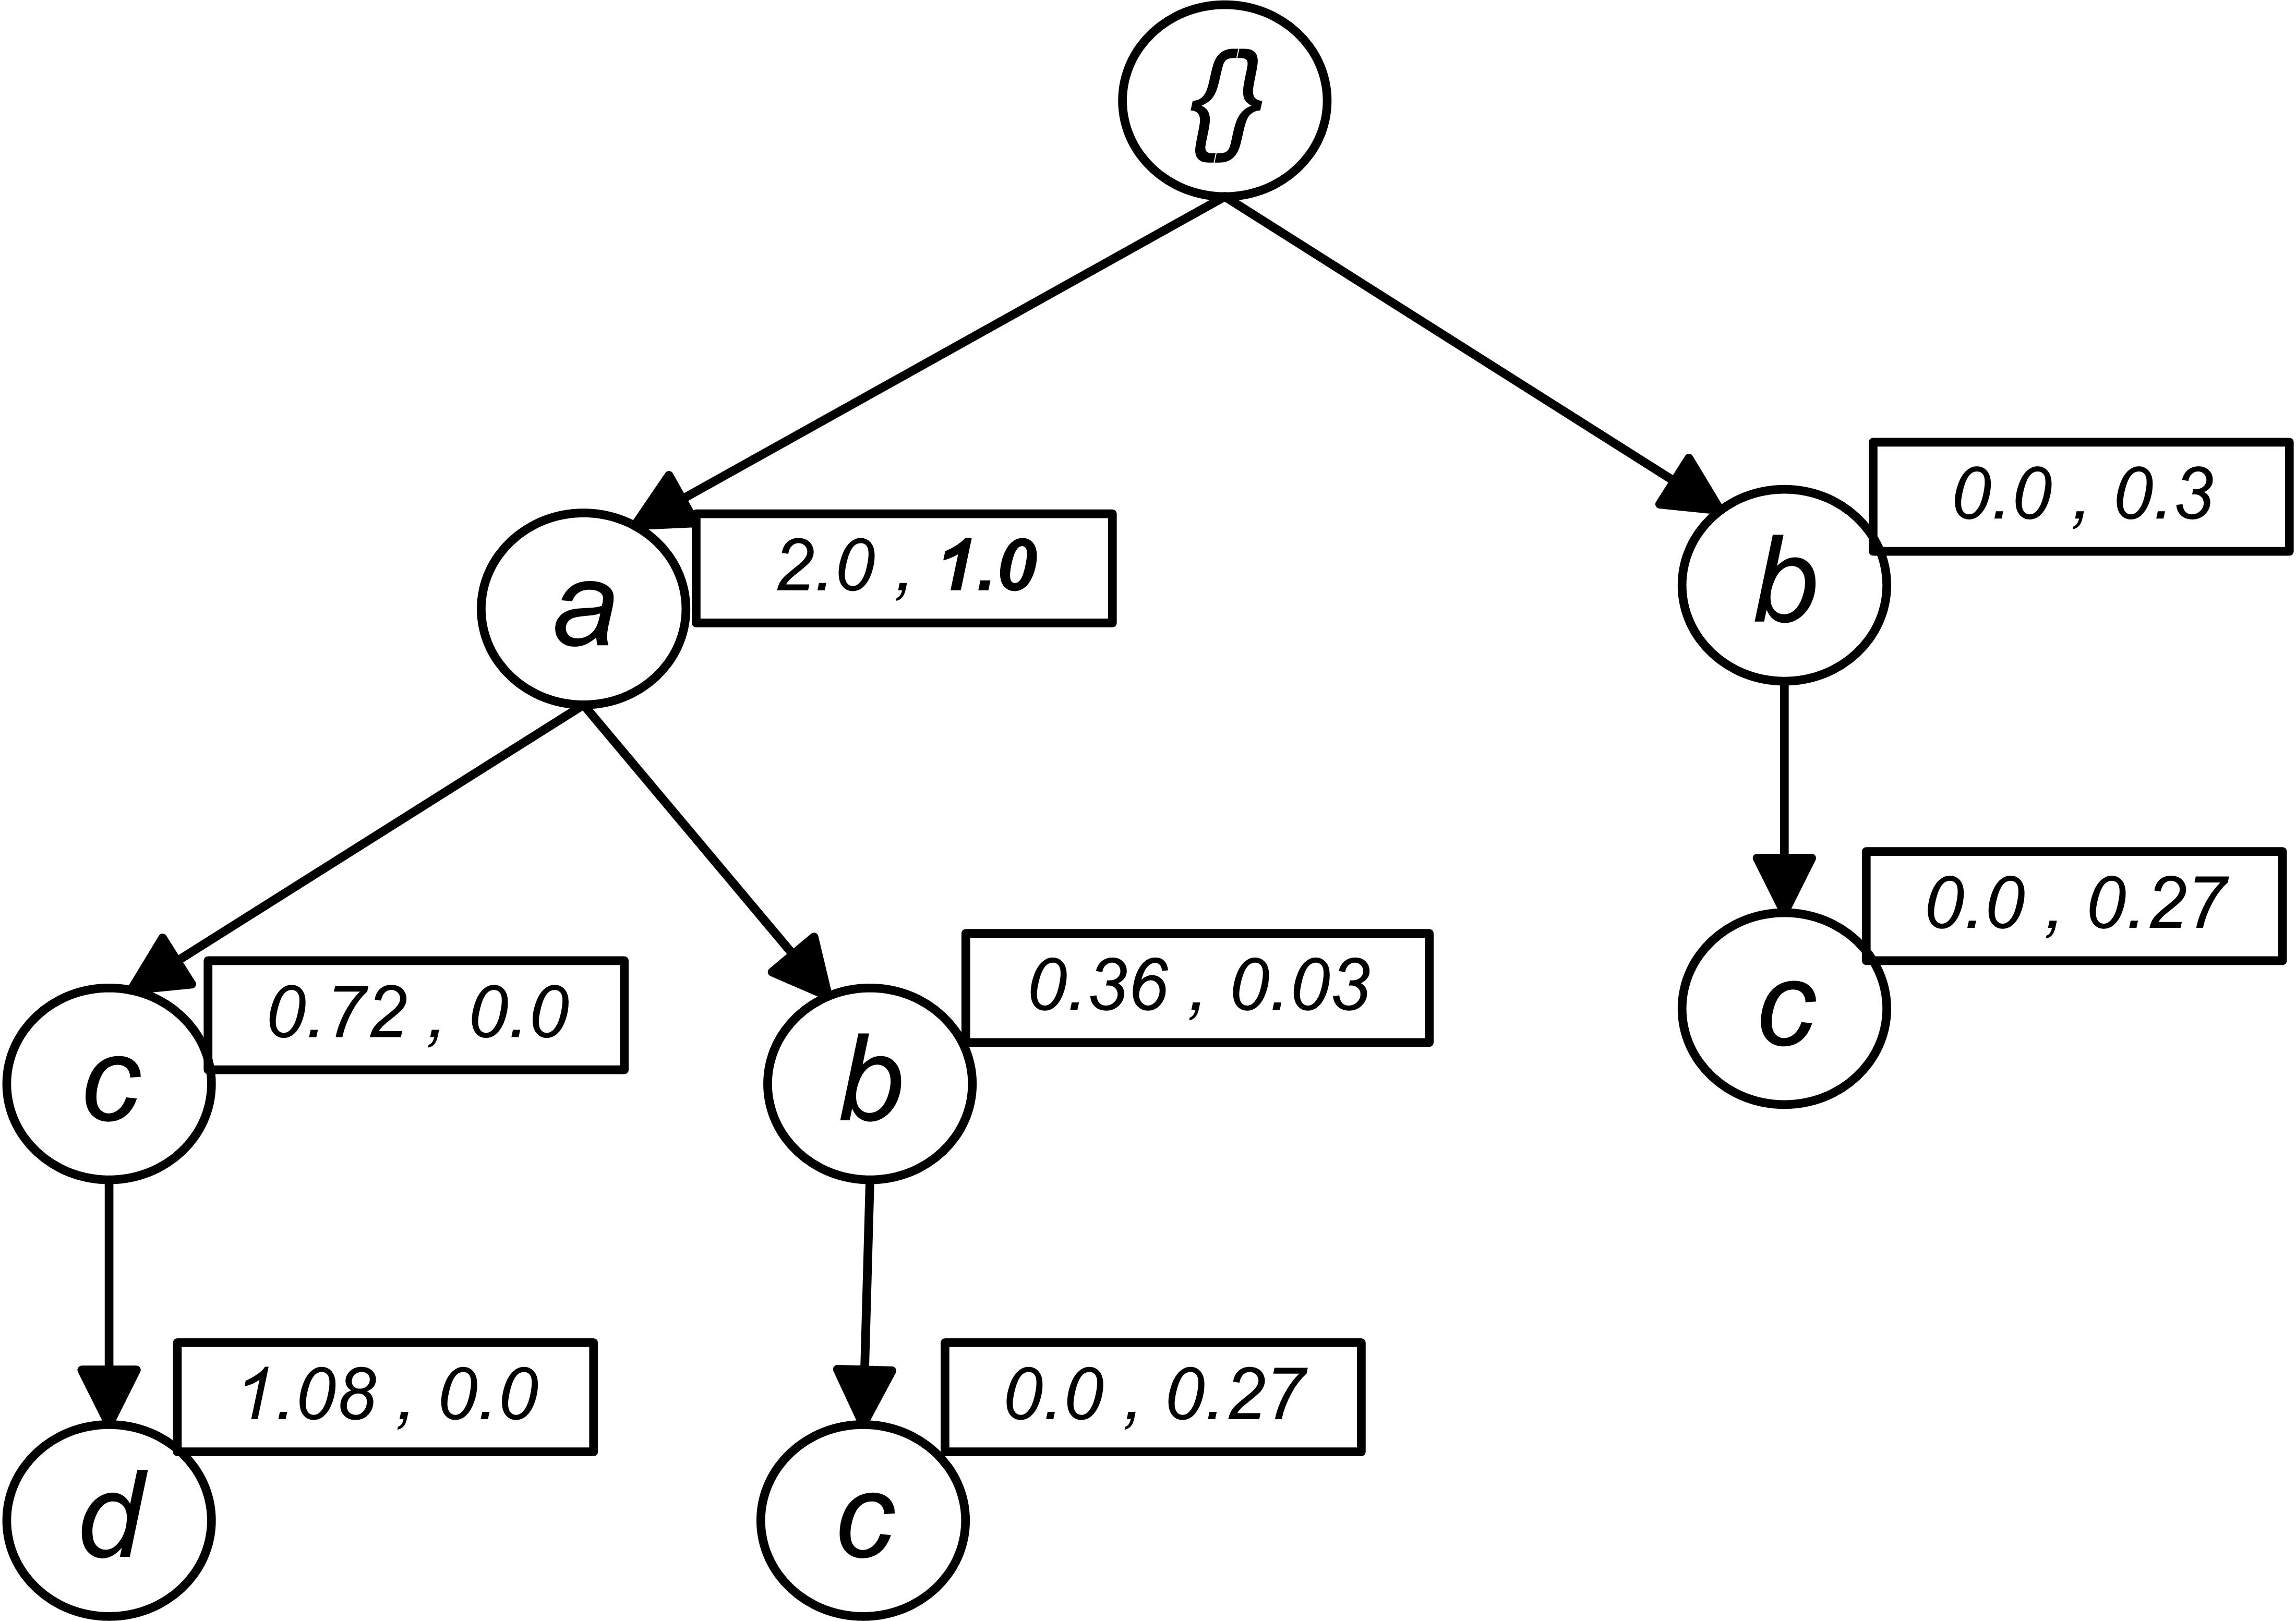
\includegraphics[width=\textwidth]{images/M_TREE.jpg}
  \captionof{figure}{US-tree for Mining}
\end{minipage}
\caption{US-tree and Header Table for Mining}
\label{figure:min_ready}
\end{figure}
%\end{document}
\paragraph{}
In this section we will discuss about our proposed approach for mining frequent pattern over large uncertain stream data. Stream Data has a special property that it comes and flows away. For this reason we will lose data after data stream has flown away. To resolve this we will proposed a window based approach where we will keep the most recent information in a tree structure as the most recent data is most valuable. Later we will show how the window will slide, remove old data and insert new data in the window. As, for uncertain data stream each same item in different transaction has different existential probability, it becomes very hard to merge (share) this node in the tree. This uncertainty property of item makes the tree huge. We have proposed a new \emph{U\textsuperscript{cap}} value for each item that helps to share a single node when constructing the tree which we named as \emph{US-tree}. We will show that our proposed tree \emph{US-tree} will be very compact and very efficient for later mining. Later will describe an approach for mining the \emph {US-tree} named \emph{USFP-growth} which is \emph{FP-growth} like approach. Later we will propose a method for filtering false positive from found most probable frequent patterns.\\ \\ \\

%\documentclass{article}
%\usepackage{caption}
%\usepackage{graphicx}
%\begin{document}
\begin{figure}
\begin{minipage}{0.40\textwidth}
  \centering
	\begin{center}
	\begin{tabular}{ |c|c| } 
 	\hline
 		Item&Value\\ \hline\hline
 		a &  1.08  	\\ \hline
 		c &  1.08   	\\ \hline
 		
\end{tabular}
\end{center}  
  \captionof{table}{\emph{d-cond tree} Header }
\end{minipage}
  \hfill
\hfill
\begin{minipage}{0.23\textwidth}
  \centering
  \hfill
  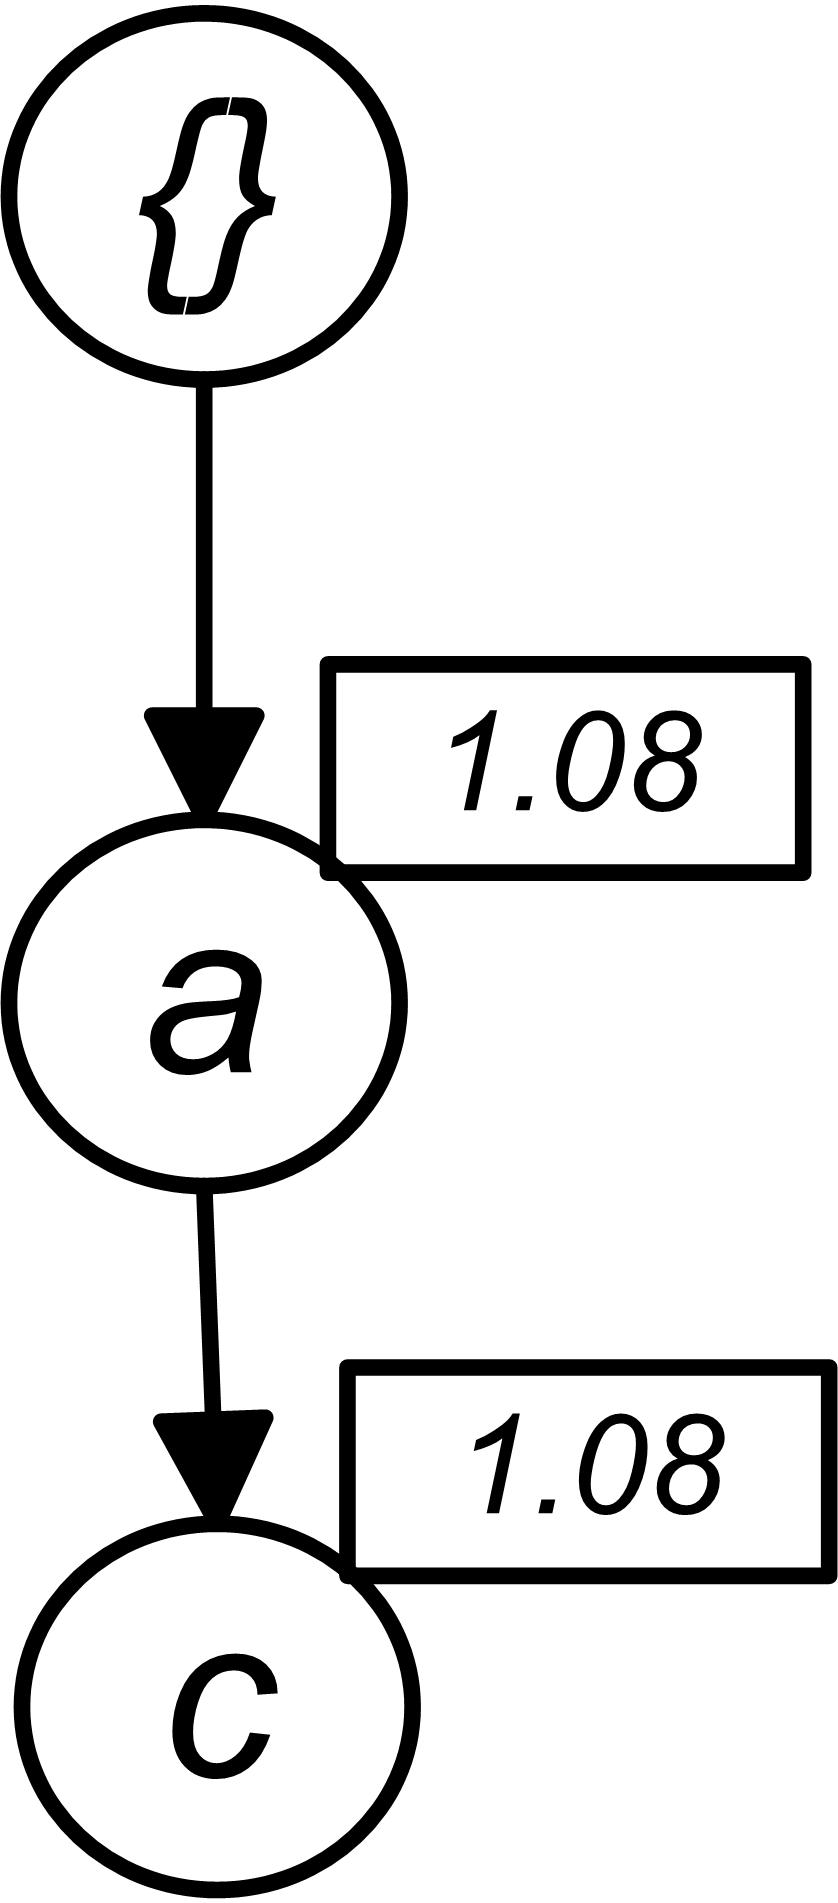
\includegraphics[width=.8\textwidth, height=5cm]{images/D_COND.jpg}
  \hfill
\end{minipage}
\hfill
\begin{minipage}{0.30\textwidth}
  \centering
  
	\begin{center}
	\begin{tabular}{ |c| } 
 	\hline
 		Freq Patterns \\ \hline\hline
 		dc  	\\ \hline
 		da   	\\ \hline
 		dca   	\\ \hline
 		
\end{tabular}
\end{center}  
  \captionof{table}{ \emph{Frequent Patterns} }
\end{minipage}
\caption{\emph{d-cond} Tree and corresponding Header}
\label{figure:d_cond}
\end{figure}
\begin{figure}
\begin{minipage}{0.30\textwidth}
  \centering
	\begin{center}
	\begin{tabular}{ |c|c| } 
 	\hline
 		Item&Value\\ \hline\hline
 		a &  .99  	\\ \hline
 		b &  .54   	\\ \hline
\end{tabular}
\end{center}  
  \captionof{table}{Header }
\end{minipage}
  \hfill
\begin{minipage}{0.29\textwidth}
  \centering
  \hfill
  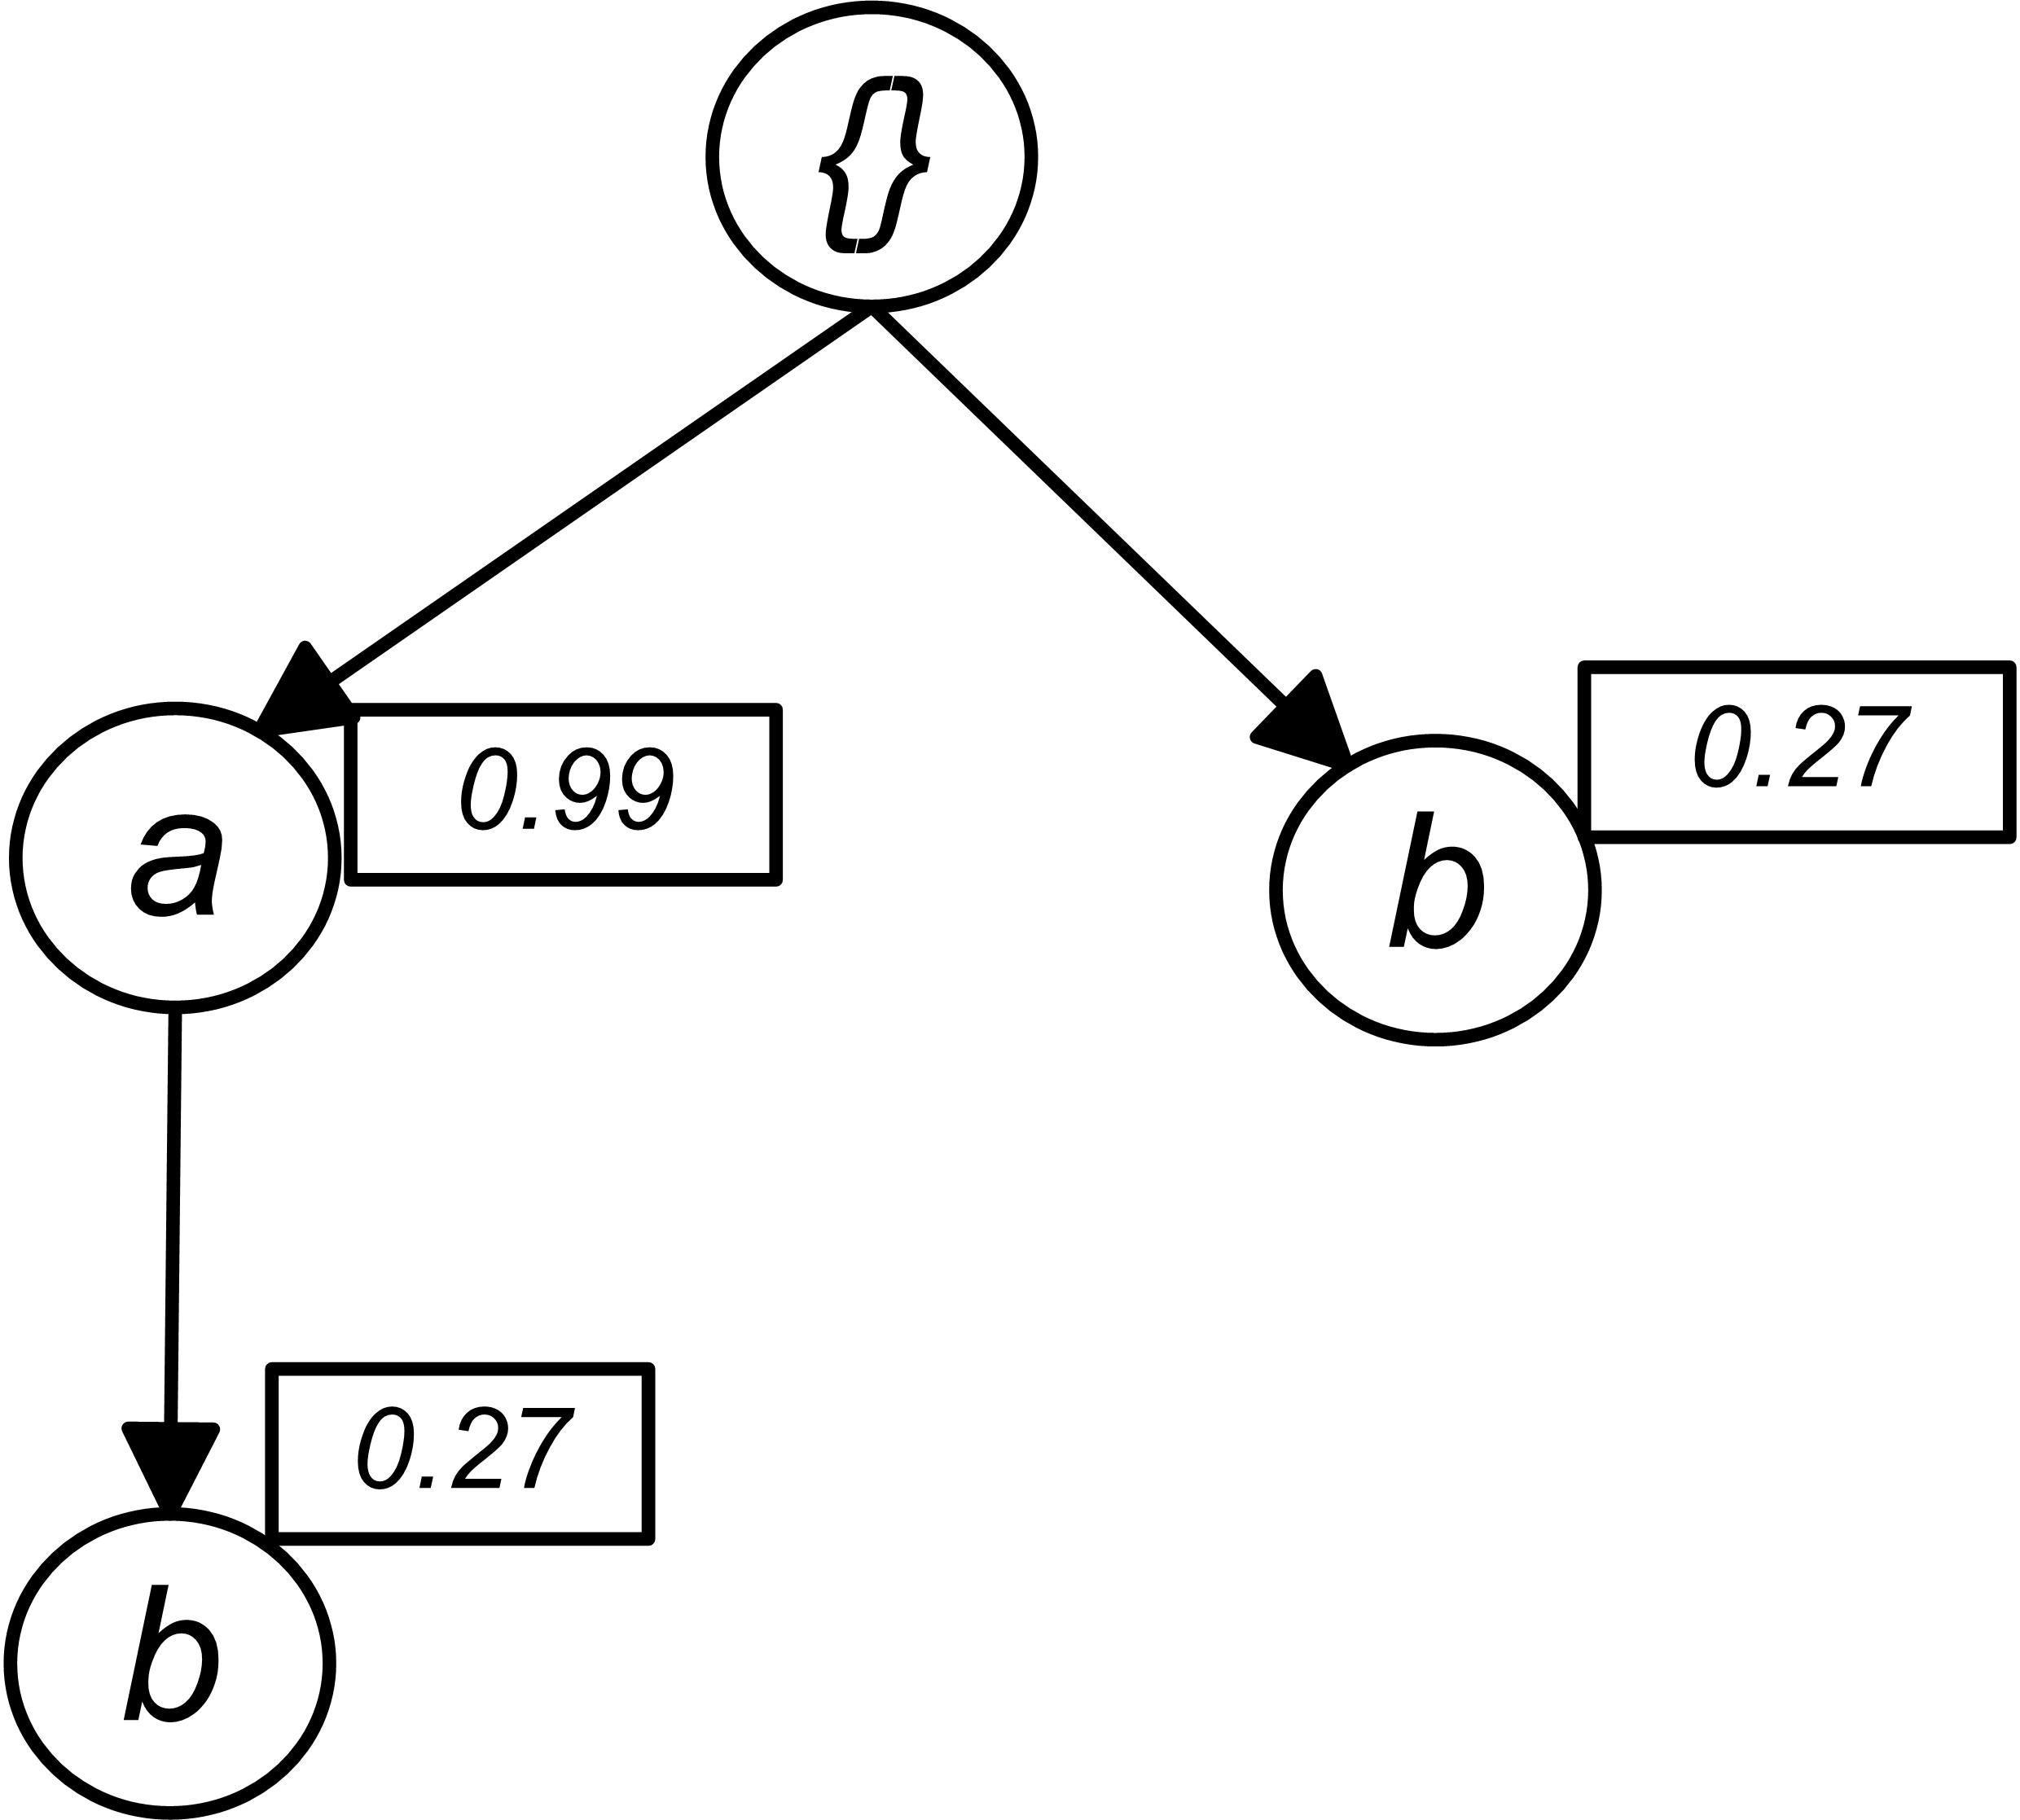
\includegraphics[width=.8\textwidth, height=3.5cm]{images/C_COND.jpg}
  \hfill  
\end{minipage}
\hfill
\begin{minipage}{0.30\textwidth}
  \centering  
	\begin{center}
	\begin{tabular}{ |c| } 
 	\hline
 		Freq Patterns \\ \hline\hline
 		ca  	\\ \hline
 		
\end{tabular}
\end{center}   
  \captionof{table}{ \emph{Freq Patterns} }
\end{minipage}
\caption{\emph{c-cond} Tree and corresponding Header}
\label{figure:c_cond}
\end{figure}
\begin{figure}
\centering
  
\includegraphics[width=.10\textwidth, height=1.1cm]{images/A_COND.jpg}
\caption{\emph{a-cond} Tree}
\label{figure:a_cond}
\end{figure}

%\end{document}


%
%\end{document}
\subsection{False positive reduction}


\paragraph{This Is Elemininition Paragraph}
%\documentclass{article}
%\usepackage{fixltx2e}
%\usepackage{caption}
%\usepackage{graphicx}
%\begin{document}
\begin{figure}
\begin{minipage}{0.40\textwidth}
  \centering
  
	\begin{center}
	\begin{tabular}{ |c| } 
 	\hline
 		Frequent Items\\ \hline\hline
 		a \\ \hline
 		b \\ \hline
 		c \\ \hline
 		d \\ \hline
 		dc \\ \hline
 		da \\ \hline
 		dca \\ \hline
 		ca \\ \hline
\end{tabular}
\end{center}  
  
  
  \captionof{table}{\emph{Frequent Items}}
\end{minipage}
\hfill
\begin{minipage}{0.40\textwidth}
  \centering
  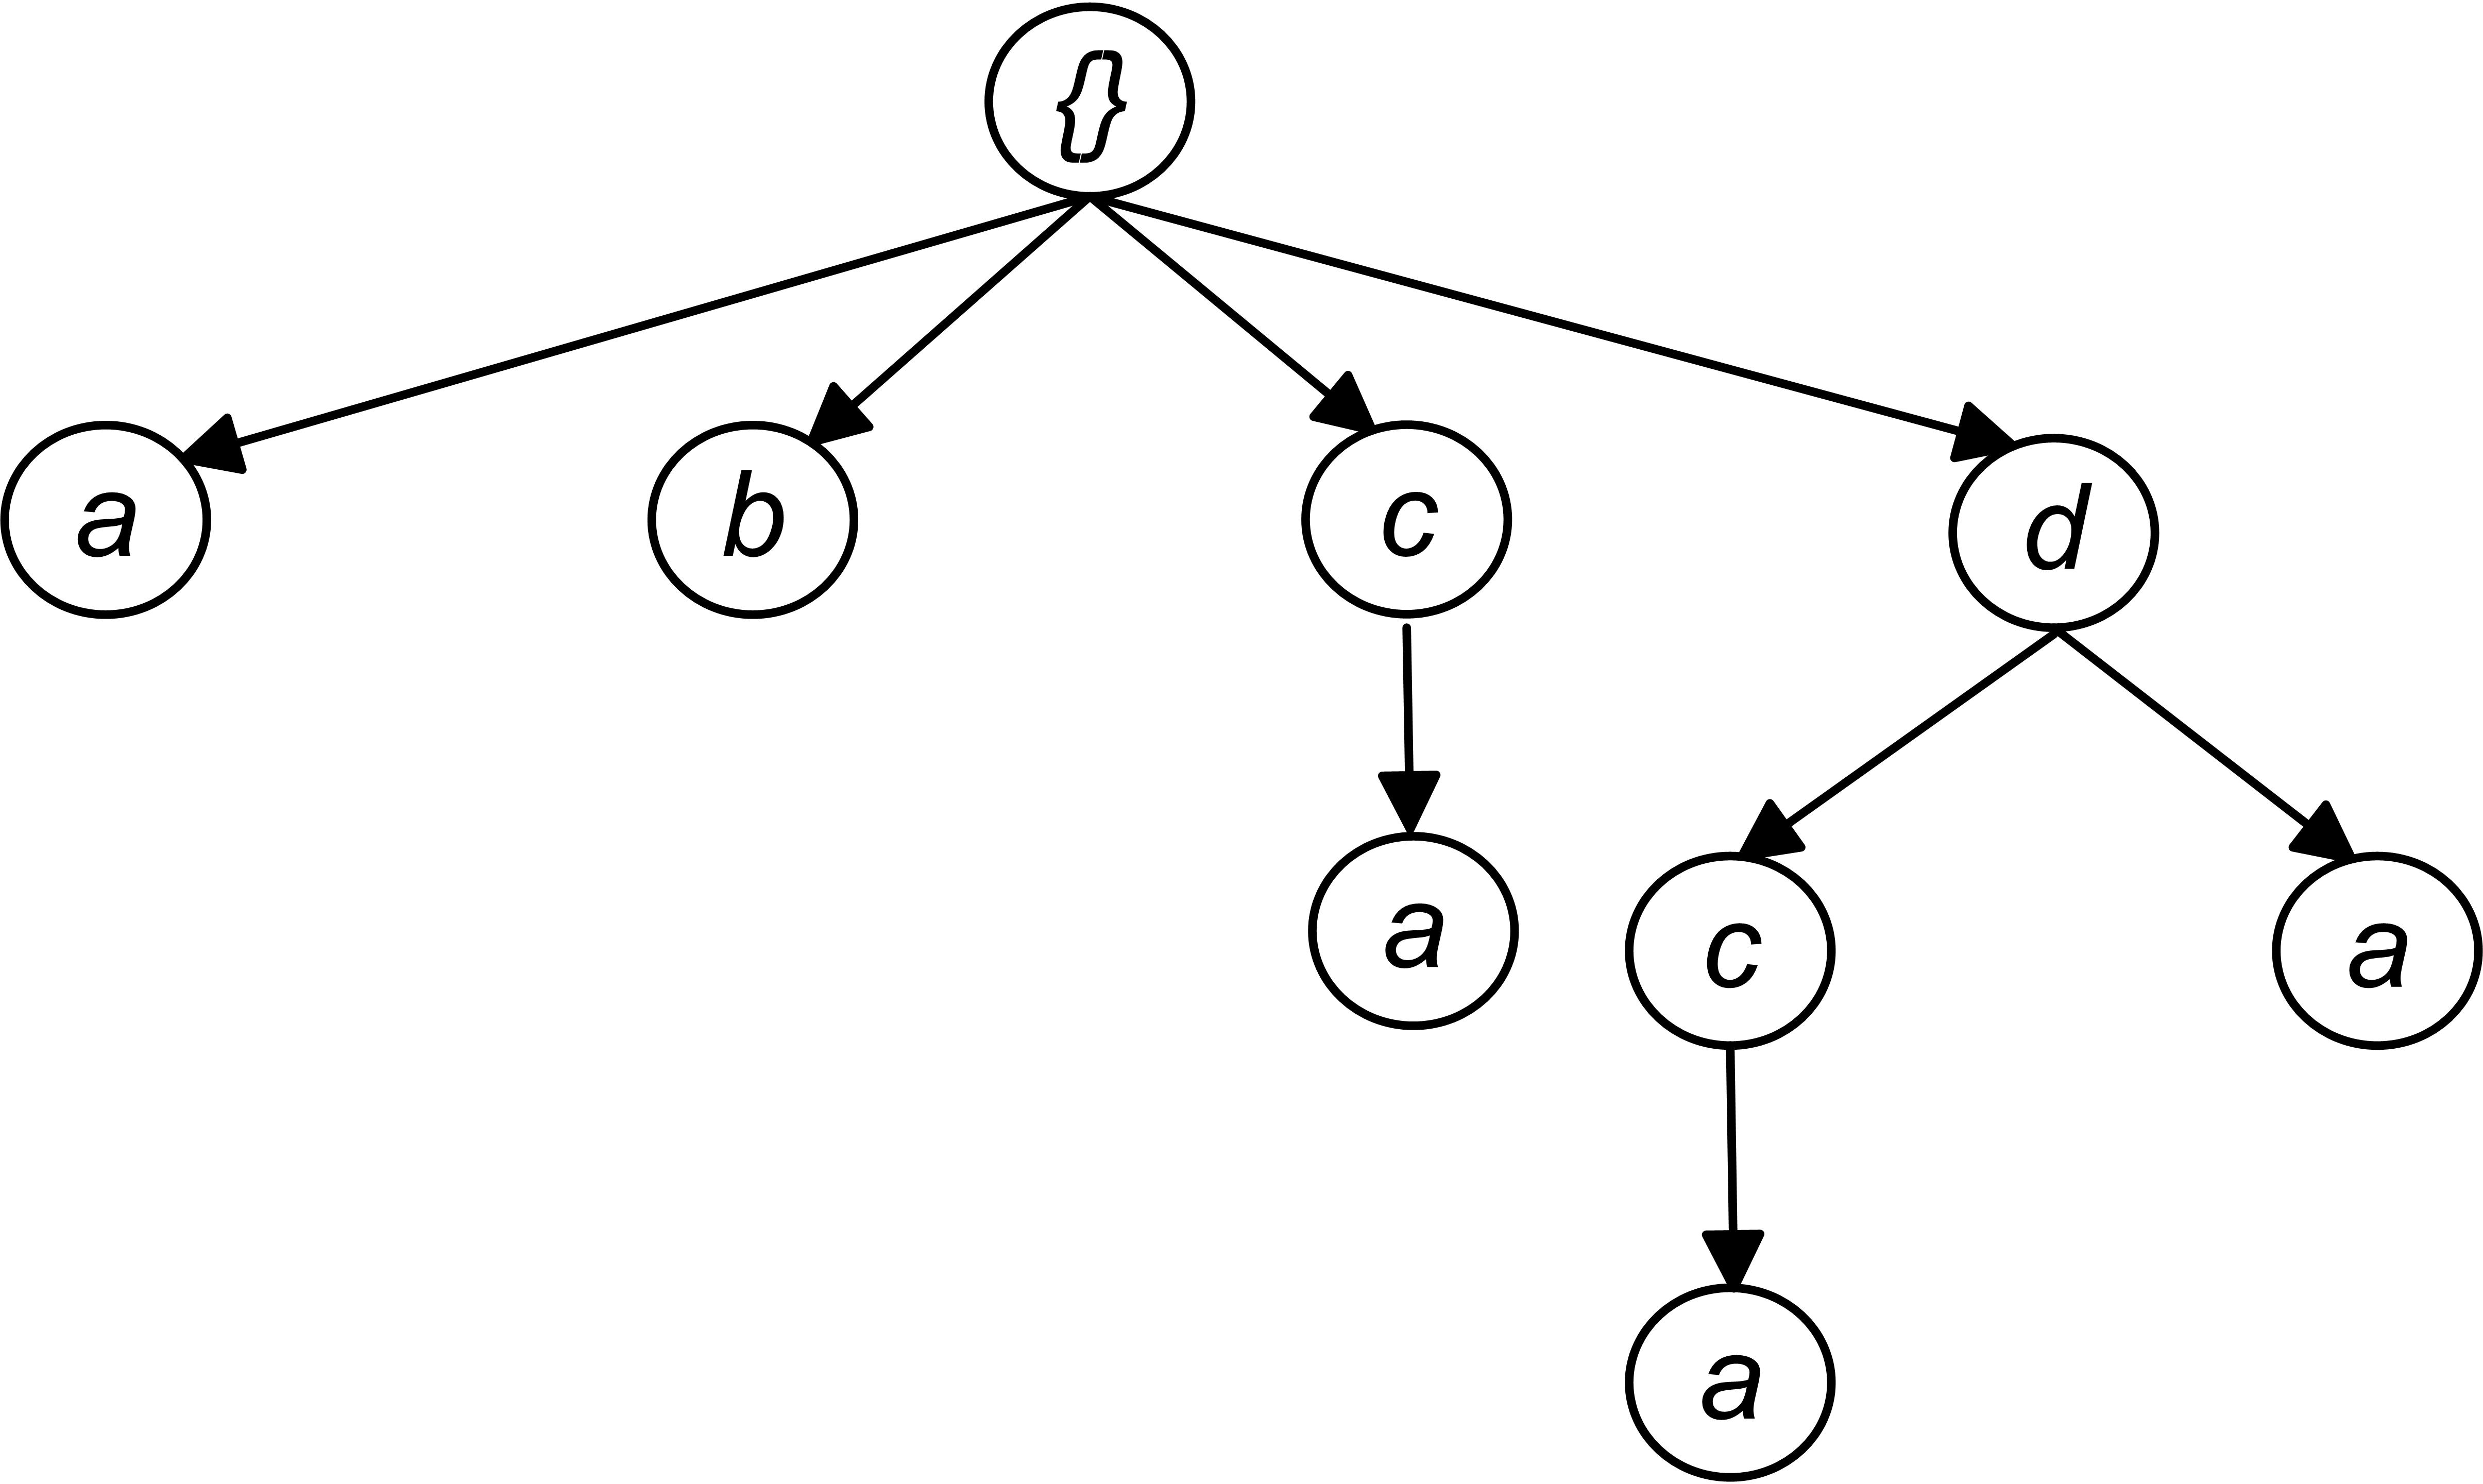
\includegraphics[width=\textwidth]{images/frequent_tree.jpg}
  \captionof{figure}{\emph{Frequent Item Tree} }
\end{minipage}
\caption{Frequent Patterns and Pattern Trees}
\label{figure:frequent_patterns}
\end{figure}
\begin{figure}
\begin{minipage}{.4\textwidth}
  \centering
  
	\begin{center}
	\begin{tabular}{ |c|c| } 
 	\hline
 		No & Items \\ \hline\hline
 		T\textsubscript{1} & \emph{a(0.9),c(0.6),d(0.5)}\\ \hline
 		T\textsubscript{2}& \emph{a(0.9),b(0.4),e(0.1)}\\ \hline
 		T\textsubscript{3}& \emph{a(0.2),c(0.9),d(0.7)}\\ \hline
 		T\textsubscript{4}& \emph{b(0.3),c(0.9)}\\ \hline
 		T\textsubscript{5}& \emph{a(0.1),b(0.3),c(0.9)} \\ \hline
 		T\textsubscript{6} & \emph{a(0.9),e(0.3)
}\\ \hline
\end{tabular}
\end{center}  
\end{minipage}
\hfill
\begin{minipage}{0.50\textwidth}
  \centering
  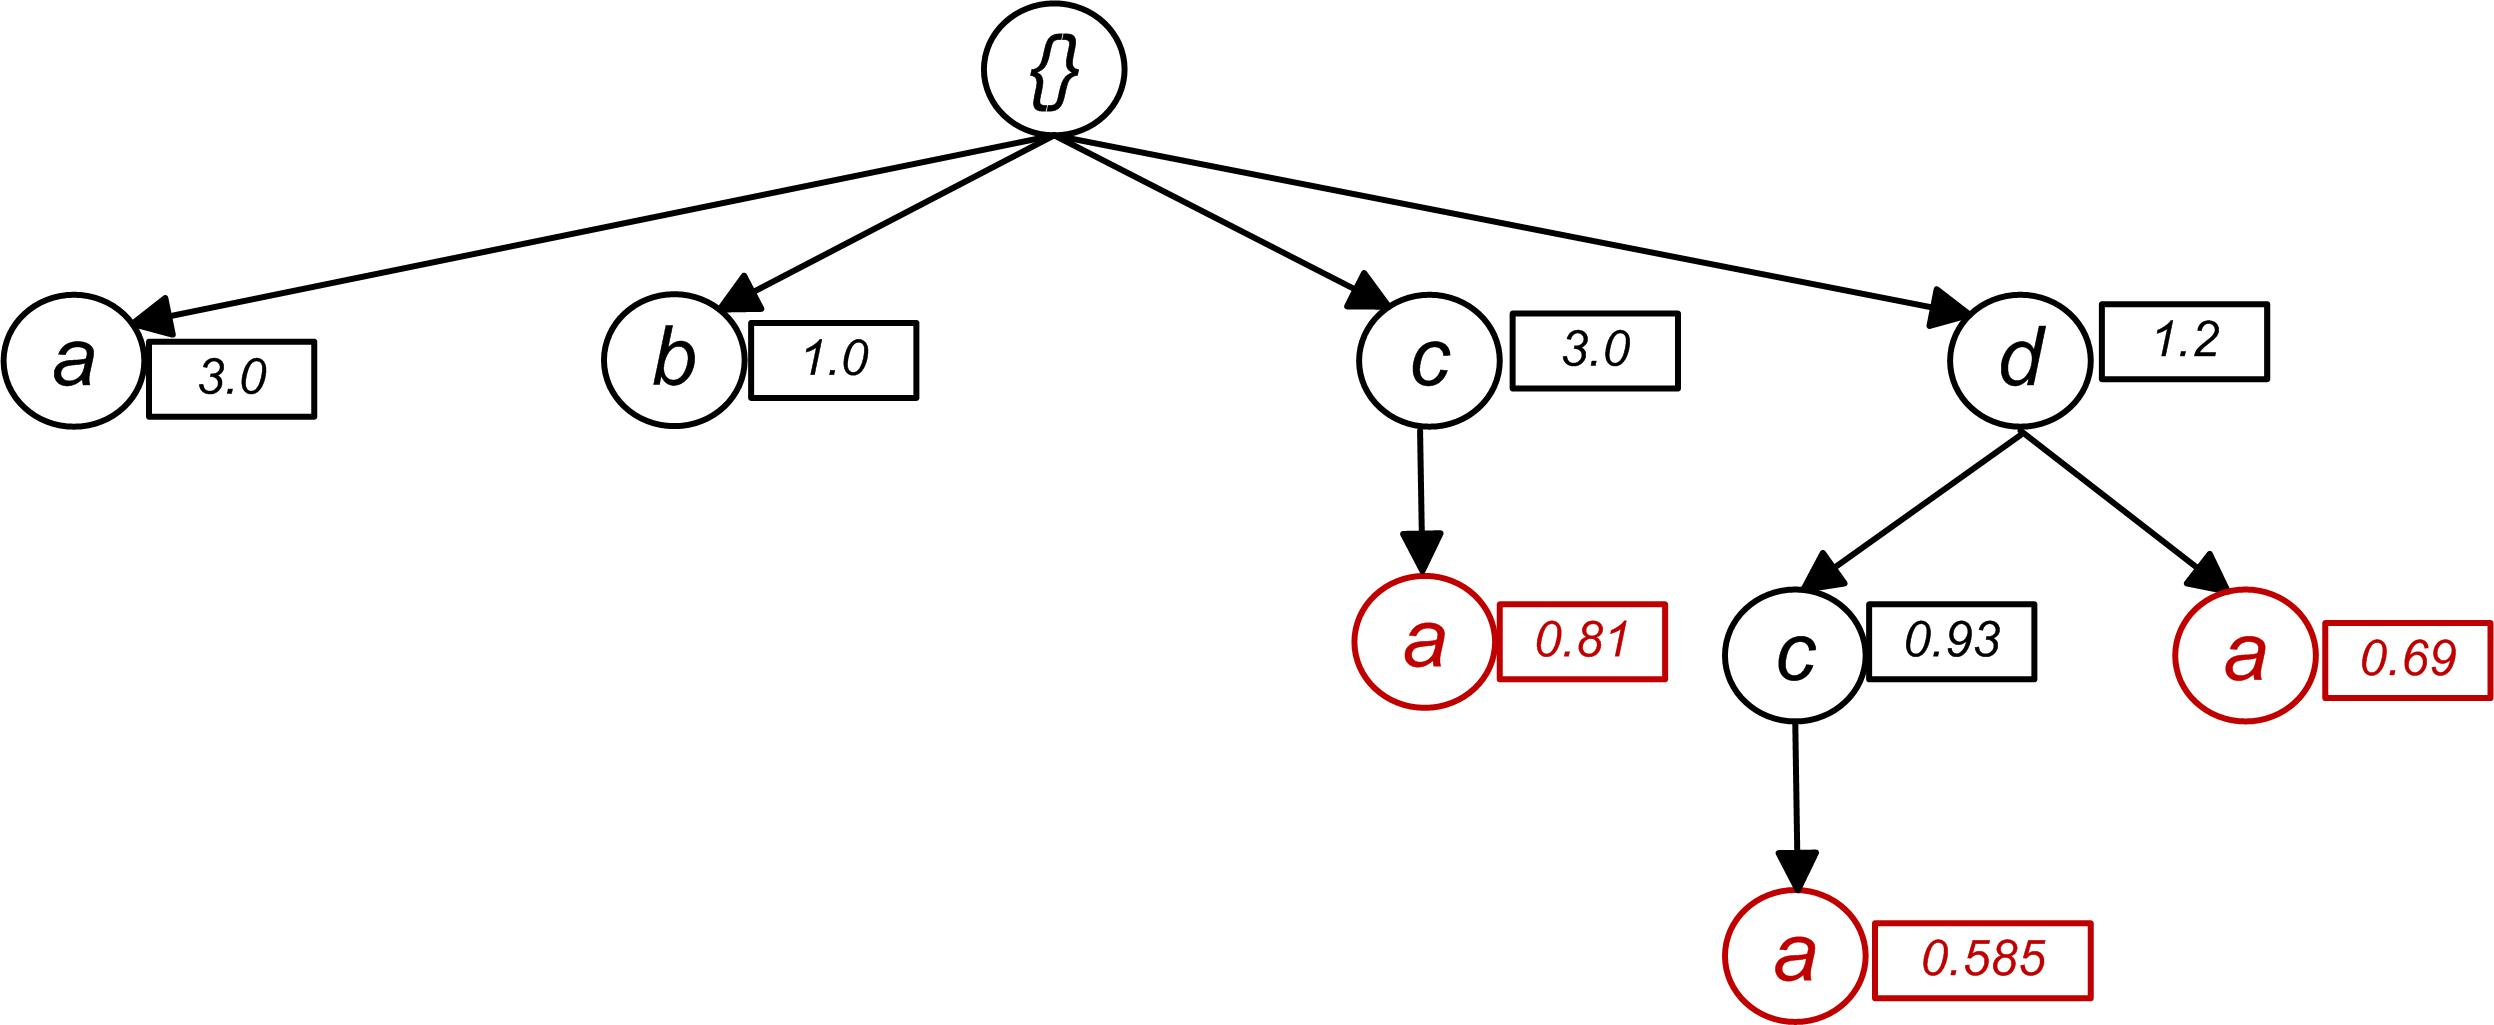
\includegraphics[width=\textwidth]{images/frequent_tree_final.jpg}
\end{minipage}
\caption{Transaction Table and Pattern Trees identifying \emph{False Positives}}
\label{figure:frequent_patterns_final}
\end{figure}
%\end{document}


\subsection{Algorithm}
%\documentclass[a4paper]{article}
%
%\usepackage[english]{babel}
%\usepackage[utf8]{inputenc}
%\usepackage{amsmath}
%\usepackage{amsfonts}
%\usepackage{graphicx}
%\usepackage[colorinlistoftodos]{todonotes}
%\usepackage{algorithm}
%\usepackage{algpseudocode}
%\usepackage{geometry}
%
%\begin{document}
\paragraph*{}
Our proposed algorithm is given here.
%\documentclass[a4paper]{article}

%\usepackage[english]{babel}
%\usepackage[utf8]{inputenc}
%\usepackage{amsmath}
%\usepackage{amsfonts}
%\usepackage{graphicx}
%\usepackage[colorinlistoftodos]{todonotes}
%\usepackage{algorithm}
%\usepackage{algpseudocode}

%\usepackage{geometry}
% \geometry{
% a4paper,
% total={210mm,297mm},
% left=20mm,
% right=20mm,
% top=20mm,
% bottom=20mm,
% }

%\begin{document}
  \begin{algorithm}
   \caption{\emph{U\textsuperscript{cap}} Assignment}
    \begin{algorithmic}[1]
      \Function{Assign\emph{U\textsuperscript{cap}}}{$Batch$ $B$}
			\For {Transaction $T$  in Batch}
				\For {$\$i=1$ to size of ( $T$ )}
					\State $\$Item$ = T[$[i]$]
					\If{$i=1$}
						\State $\$Item$[\emph{U\textsuperscript{cap}}] $=$ $Probability(\$Item)$
					\Else
						\State $\$Item$[\emph{U\textsuperscript{cap}}] $=$ MAX \{ $Probability(\$T[1])$ to $Probability(\$T[i-1])$ \} $*$ $Probability(\$Item)$
					\EndIf
				\EndFor
			\EndFor
       \EndFunction

\end{algorithmic}
\end{algorithm}
%\end{document}
%\documentclass[a4paper]{article}
%
%\usepackage[english]{babel}
%\usepackage[utf8]{inputenc}
%\usepackage{amsmath}
%\usepackage{amsfonts}
%\usepackage{graphicx}
%\usepackage[colorinlistoftodos]{todonotes}
%\usepackage{algorithm}
%\usepackage{algpseudocode}
%
%
%\begin{document}
%\listoffigures
\begin{enumerate}

 \item Some text goes here . . .
  \begin{algorithm}
   \caption{Merge Sort}
    \begin{algorithmic}
      \Procedure{Merge}{$A,p,q,r$}\Comment{Where A - array, p - left, q - middle, r - right}

        \State ${n_1} = q - p + 1$
        \State ${n_2} = r - q$
        \State Let $L[1 \ldots {n_1} + 1]$ and $R[1 \ldots {n_2} + 1]$ be new arrays
        \For{$i = 1$ to ${n_1}$}
            \State $L[i] = A[p + i - 1]$
        \EndFor
        \For{$j = 1$ to ${n_2}$}
            \State $R[i] = A[q + j]$
        \EndFor
        \State $L[{n_1} + 1] =  \infty $
        \State $R[{n_2} + 1] =  \infty $
        \State $i = 1$
        \State $j = 1$
        \For{$k = p$ to $r$}
            \If {$L[i] < R[j]$}
                \State $A[k] = L[i]$
                \State $i = i + 1$
            \ElsIf {$L[i] > R[j]$}
                \State $A[k] = R[j]$
                \State $j = j + 1$
            \Else
                \State $A[k] = - \infty$ \Comment{We mark the duplicates with the largest negative integer}
                \State $j = j + 1$
            \EndIf
        \EndFor
       \EndProcedure

\end{algorithmic}
\end{algorithm}
\end{enumerate}
%\end{document}
%\documentclass[a4paper]{article}
%
%\usepackage[english]{babel}
%\usepackage[utf8]{inputenc}
%\usepackage{amsmath}
%\usepackage{amsfonts}
%\usepackage{graphicx}
%\usepackage[colorinlistoftodos]{todonotes}
%\usepackage{algorithm}
%\usepackage{algpseudocode}
%
%
%\begin{document}
%\listoffigures
\begin{enumerate}

 \item Some text goes here . . .
  \begin{algorithm}
   \caption{Merge Sort}
    \begin{algorithmic}
      \Procedure{Merge}{$A,p,q,r$}\Comment{Where A - array, p - left, q - middle, r - right}

        \State ${n_1} = q - p + 1$
        \State ${n_2} = r - q$
        \State Let $L[1 \ldots {n_1} + 1]$ and $R[1 \ldots {n_2} + 1]$ be new arrays
        \For{$i = 1$ to ${n_1}$}
            \State $L[i] = A[p + i - 1]$
        \EndFor
        \For{$j = 1$ to ${n_2}$}
            \State $R[i] = A[q + j]$
        \EndFor
        \State $L[{n_1} + 1] =  \infty $
        \State $R[{n_2} + 1] =  \infty $
        \State $i = 1$
        \State $j = 1$
        \For{$k = p$ to $r$}
            \If {$L[i] < R[j]$}
                \State $A[k] = L[i]$
                \State $i = i + 1$
            \ElsIf {$L[i] > R[j]$}
                \State $A[k] = R[j]$
                \State $j = j + 1$
            \Else
                \State $A[k] = - \infty$ \Comment{We mark the duplicates with the largest negative integer}
                \State $j = j + 1$
            \EndIf
        \EndFor
       \EndProcedure

\end{algorithmic}
\end{algorithm}
\end{enumerate}
%\end{document}
%\end{document}
\section{Summary}
\noindent
In this section we will discuss about our proposed approach for mining frequent pattern over large uncertain stream data. Stream Data has a special property that it comes and flows away. For this reason we will lose data after data stream has flown away. To resolve this we will proposed a window based approach where we will keep the most recent information in a tree structure as the most recent data is most valuable. Later we will show how the window will slide, remove old data and insert new data in the window. As, for uncertain data stream each same item in different transaction has different existential probability, it becomes very hard to merge (share) this node in the tree. This uncertainty property of item makes the tree huge. We have proposed a new \emph{U\textsuperscript{cap}} value for each item that helps to share a single node when constructing the tree which we named as \emph{US-tree}. We will show that our proposed tree \emph{US-tree} will be very compact and very efficient for later mining. Later will describe an approach for mining the \emph {US-tree} named \emph{USFP-growth} which is \emph{FP-growth} like approach. Later we will propose a method for filtering false positive from found most probable frequent patterns.
%%\documentclass{article} 
%\usepackage{graphicx}  
%\usepackage{multirow}
%\usepackage[table]{xcolor}
%\usepackage{fixltx2e}
%\usepackage{array}
%
%\begin{document}
\begin{table}[ht]
\centering

\begin{tabular}{|c|c|c|c|c|c|}
\hline
	Transaction No & \multicolumn{4}{c|}{Items in Transaction} \\ \hline \hline
	T\textsubscript{1} & a(0.9) & c(0.6) & d(0.5) & e(0.2)			\\\hline
	T\textsubscript{2} & a(0.9) & b(0.4) & e(0.1) & --    			\\\hline
	T\textsubscript{3} & a(0.2) & c(0.9) & d(0.7) & --    			\\\hline
	T\textsubscript{4} & b(0.3) & c(0.9) & -- & --			\\\hline
	T\textsubscript{5} & a(0.1) & b(0.3) & c(0.9) & --    			\\\hline
	T\textsubscript{6} & a(0.9) & e(0.3) & -- & --        			\\\hline
   	T\textsubscript{7} & a(0.1) & d(0.6) & e(0.2) & --		\\\hline
	T\textsubscript{8} & a(0.1) & c(0.2) & f(0.6) & --    			\\\hline
	T\textsubscript{9} & c(0.2) & d(0.9) & f(0.6) & --    			\\\hline
	
	T\textsubscript{10} &  --  &  --  &  --  & --    				\\\hline
	T\textsubscript{11} &  --  &  --  &  --  & --    				\\\hline
	T\textsubscript{12} &  --  &  --  &  --  & --    				\\\hline
	
		
\end{tabular}
\label{tab:ex_u}
\caption{Example of Uncertain Stream Transaction}
\label{table:uncertain_stream_transaction}
\end{table}
%\end{document}

\end{document}